% ============================================================
%  第九卷 第六章（后半） 晶格中的电子（§62–§68）
%  底本：高教社中文第4版（王锡绂 译）；印刷页 240–264（PDF p251–p275）
%  不带 \chapter（章头在 ch06a.tex），自 \section{金属中电子的格林函数} 起
%
%  插图清单：编号插图 2 幅，重绘 figures/fig15.pdf、fig16.pdf 已就位：
%    图 15（p257，费米面哑铃形极值截面，场方向箭头；图注原书仅"图 15"）
%    图 16（p260，H(B) 麦克斯韦构造回线（ab/bc/cd/ad，阴影面积相等）；
%           图注原书仅"图 16"）
%  两图原书均随文右栏排布，此处按原子图块置于就近段后（minipage 防跨页）。
%  图 14（p237）属 ch06a 范围，不在本文件。
%
%  图式等式：§64 共 3 处（(64.5) 电子格林函数一级修正；（64.7）声子格林
%  函数一级修正；（64.9）电子-声子顶角），全部用 picture 环境按页面
%  p261/p262 重绘（外线标号 P/K/P−K/P₁′=P₁+K/P₂′=P₂−K、虚/实线、箭头
%  方向逐图对照页面）；(64.5) 声子弧按页面排虚线（qbezier 分段）。
%
%  圈码脚注：正文圈码共 34 处原位保留（p253①②、p254①②、p255①、
%  p256①、p257①、p258①②、p259①、p260①②、p261①②、p263①②③、
%  p265①、p266①、p267①②、p268①、p269①②、p270①、p271①②③、
%  p272①②、p273①、p274①、p275①②）。脚注文本未转录，待脚注代理
%  按页面 PNG 页脚补录。OCR 窜入正文的一块脚注公式（p257①之积分值）
%  已挪出为 %%FN 注释。
%
%  编号公式核算：OCR 带 tag 65 条；(64.5)(64.7)(64.9) 页面带编号而 OCR
%  为图块，按 equation 自动编号补齐。故本文件编号公式共 68 个：
%  §62 9、§63 18、§64 11（含图式 3）、§65 13、§66 3、§67 7、§68 7。
%  逐节与页面核对无重号、无缺号、无跳号。文件头 \setcounter{section}{61}
%  保证单独编译时节号/公式号与原书一致（全书连排时 ch06a 已至 §61，
%  该行幂等无害）。
%
%  已修正的 OCR 错误（均对照 原书转换/pages/pNNN.png 逐条核实）：
%   1. §62 首段（p251）：引文按页面为"[Ю. А. Бычков, Л. П. Горьков,
%      1961; J. M. Luttinger, 1961)"（西里尔，括号不配对接页面照排，
%      见排印问题 a）；"引人"→"引入"；OCR 乱序之"断言/r₁−r₂/下面"理顺；
%      "T=\dot 0"按页面为 T=0（0 上墨点为噪声）；段末孤立"2"为噪声删除；
%      破折号"———0态——"按页面为"——0态——"。
%   2. (62.1)(62.2)（p252）：OCR r_\lfloor 之类按页面为 r₁；(62.2) 第二式
%      下标按页面照排为 αm,k（无负号，见排印问题 b）。
%   3. (62.3)（p252）：OCR \lfloor 系 r₁ 误识；分母 ε^{(±)}_{mk} 上下标
%      按页面恢复；求和号下标 m,k 之 k 按页面为粗体。
%   4. §62 自能函数（p252）：OCR "Σ_αβ(τ, r₁, r₂)"按页面为
%      Σ_αβ(t, r₁, r₂)；(62.5) OCR "∫ dΣ"按页面为 ∫Σ_αγ(…)d³x′
%      （体积元按页面照排 d³x′）。
%   5. (62.6)（p253）：OCR \sum_{αγ}按页面为大写 Σ_{αγ}；"根据
%      ω=ε(r)−μ"照页面排 ε(r)（疑为 ε(k)，见排印问题 c）。
%   6. (62.7)（p253）：OCR \mathcal K 按页面为粗斜体 K（\bm K）。
%   7. (62.9) 后段（p254）：OCR "对于 k_z 电子费米液体"按页面为
%      "对于金属电子费米液体"；ξ(k_z) 记号理顺；"量子化"按页面为黑体。
%   8. §63（p254–p255）：节名按页面"迪·哈斯-范·阿耳芬效应"；
%      "(.M.，A. M. K,1955)"按页面为"(И. М. Лифшиц, А. М. Косевич,
%      1955)"（西里尔）；"de Haas vanAlphen"补空格；
%      "[比较222页上的注释)"括号按页面为"]"。
%   9. (63.3)–(63.8)（p255–p256）：\widetilde Ω 记号统一；(63.5) 分母按
%      页面照排 4π²cℏ（(63.3) 为 4π²ℏc）；(63.6) e^{2πiln} 之 ln 为 l·n；
%      (63.8) ∂n/∂ε 位置按页面。
%  10. p256 鞍点诸式：n(ε,k_z)≈… 中 OCR 之 k_ε 按页面为 k_z；贡献式
%      \frac{dn_ex}{dε√l}|…|^{-1/2} 按页面重建；"在指数函数中指数的
%      ＋导和－号"照页面照排（"导"疑为"号"，见排印问题 d）；
%      (63.9) 分母指数按页面照排为 2（见排印问题 e）。
%  11. p257：OCR 窜入正文的脚注公式块 I≡∫e^{iαz}dz/(e^z+1)=−iπ/sinhπα
%      挪出为 %%FN 注释；arsinh 诸式按页面照排；(63.10) 双"×"续行按页面。
%  12. (63.11)（p257–p258）：三行右花括号系统按页面排；Ω_l 分母
%      π^{7/2}ℏ³m*l^{5/2}、λ=lπ²Tm*/mβB 逐项核对。
%  13. (63.12)–(63.13)（p258）："因子一余弦"按页面为"因子—余弦"；
%      (63.13) OCR "et'"、"±k_ex"乱码按页面为 M̃_z 与
%      cos(πl(m*/m)ξ_ex)；M_l 分母 π^{7/2}m*l^{3/2}ℏ。
%  14. p259：OCR "M,原则上"按页面为"M̃，"；"[因 M̃/B∼…]"按页面为
%      "[因为 M̃/B∼χ̄(μ/βB)^{1/2}]"；"Ω̃γΩ₀"按页面为"Ω̃/Ω₀"；
%      "υo)"、"v_r"按页面为 v_F^{(0)}、v_F；"$;v_F$"窜入位移理顺；
%      (63.18) 左端 |χ̄| 照页面（见排印问题 g）。
%  15. p260：OCR B_\alpha 按页面为 B_a；"\mathcal Q"为圈码②；
%      外场哥特体记号统一为 \mathfrak H；"抗磁畴"按页面黑体。
%  16. §64（p260–p262）：(64.1) OCR "U_{KT}"乱码按页面为 U_形变（汉字
%      下标）；正文 "U_{##}"同；(64.2) OCR "H_{∥∥}"按页面为 Ĥ_电声；
%      (64.6) OCR "\mathfrak d"按页面为 δ；(64.8) "8"→δ；
%      (64.10) OCR {\cal T} 按页面为 Γ；正文"ω_p"按页面为 ω_D；
%      (64.9) 外线标号 P₁′=P₁+K、P₂′=P₂−K 按页面。
%  17. §65（p263）：OCR "vg的上标(0)"按页面为"v_F 的上标(0)"（位移理顺）；
%      (65.2) OCR "\dot G"按页面为 G^{(0)}；"散射幅"照页面用字。
%  18. p264：{⋯} 式行末"sign(ε−−μ−ω)"为原书断行重影，按 sign(ε−μ−ω)
%      排（整理，登记为排印问题 j）；(65.5) OCR "\iint^{ε−μ1}"按页面为
%      ∫_0^{|ε−μ|}；估计段"参量 v_F^{(0)} 和 ω 起源于电子"按页面"和"后
%      为 w（斜体 w），其后公式"ω∼ε_F∼ℏ²/ma²"照页面（见排印问题 k）。
%  19. (65.11)（p265）：分子按页面照排 Zω²（疑为 Zw²，见排印问题 l）；
%      (65.12) OCR "\stackrel{≡}"乱码按页面为"当 ε−μ≫ℏω_D"。
%  20. §65 习题（p266）：iδD^{−1} 乱码按页面重建（右端 −2w²/ρ²）；
%      OCR "\mathfrak E"→δ；α 式分母 4πℏ³ρuv_F²；ρu∝√M。
%  21. §66（p267–p268）：ε_s(k) OCR "ε,(k)"→ε_s(k)；"单在任何情况下…"
%      句按页面补齐"个电子(或空穴)的衰减在能量最小值上方的有限间隔内
%      严格等于零②. 事实上，在任何情况下…"（OCR 脱文）；"能隙 Δ 参阅"
%      补逗号；OCR "电 J^x 子"按页面为"电子"；"最大束缚 ∆_− 能)"按页面
%      为"最大束缚能)"；"(…束缚能数 1/ε ε 量级的频率值)"按页面为
%      "(…束缚能数量级的频率值)"；"能量的最小值 k=0 处"按页面补"在"。
%  22. §67（p269–p271）："m_ℏ"按页面为 m_h；(67.3)–(67.7) 逐项核对；
%      化学反应式按页面"e+h⇌0"；代换式长箭头恢复；OCR E_eb 按页面为
%      E_eh；(67.2) 后"为了明确起见."句读照页面。
%  23. §68（p271–p274）：(68.1) γ̂_{ik} 粗体戴帽按页面；ψ₂ 式按页面
%      照排"x²+ω²y²+ωz"（疑漏平方，见排印问题 n）；γ 矩阵元按页面重建
%      （⟨1|γ_xx|2⟩=⟨2|γ_xx|1⟩≡B；⟨1|γ_zz|2⟩=ω²B，OCR γ_z→γ_zz）；
%      D_u′(或 D_g′) 之 OCR "D_B′"→D_g′；基底矩阵行按页面重建为
%      ĵ_x, ĵ_x², {ĵ_x,ĵ_y}_+, ĵ_x³, {ĵ_x,ĵ_y²−ĵ_z²}_+（OCR 混乱）；
%      (68.3) OCR 之 k_s 按页面为 k_x/k_y；(68.4) 五行按页面照排
%      （含 V₁₂=−V₃₄=(√3/2)β₃k_x(k_y+ik_x)）；(68.4) 后"克拉默斯型"照
%      页面；λ 式、(68.6)、A/B/C、(68.7) 逐项核对。
%  24. §68 末段（p275）：OCR 乱序"成一个点 k₀. T=0 时"理顺，衍"k₀"删除；
%      "无能隙半导体"按页面黑体。
%  25. 全章：\pmb→\bm；偏导 ∂ 恢复；sign/Re/Im/exp/arsinh 正体；d 微分
%      正体；p259 "以M标 M̄ 记"按页面为"（以 M̄ 标记）"；圈码①位于公式
%      内部者（χ=δM/δH①）移出公式置于其后。
%
%  原书排印问题（照排并登记，供总校裁定）：
%   a. p251：引文括号不配对"[Ю. А. Бычков, …, Luttinger, 1961)"，照排。
%   b. p252：(62.2) 第二式下标印作 αm,k，与 (62.1) 之 αm,−k 不一致
%      （且两式均为 e^{ik·r}），照排。
%   c. p253："根据 ω=ε(r)−μ"之 ε(r) 疑为 ε(k)（比较 (62.4) 极点位置），
%      照排。
%   d. p256："指数的＋导和－号"之"导"疑为"号"，照排。
%   e. p256：(63.9) 分母 |∂²n/∂k_z²|²_ex 与 (63.10) 之 |·|^{1/2}_{ex,μ}
%      不一致，照排。
%   f. p257：(63.10) 之 arsinh 因子与 (63.11) 之 λ/sinhλ 并存，与脚注
%      积分值 ∝1/sinh πα 的量纲关系存疑，照排。
%   g. p259：(63.18) 左端 |χ̄| 按上下文（振荡部分之模）疑为 |χ̃|，照排。
%   h. p262："|ε−ε_F|≪ω_D"疑漏 ℏ（比较前文 ℏω_D），照排。
%   i. p263："Σ=G^{(0)−1}−ε^{−1}"之 ε^{−1} 疑为 G^{−1}，照排。
%   j. p264：{⋯} 式因断行出现"sign(ε−−μ−ω)"重影负号，重排时按
%      sign(ε−μ−ω) 排（本条为整理，非照排）。
%   k. p264："ω∼ε_F∼ℏ²/ma²"之 ω 疑为 w（与注脚 w∼ε_F 及本段首句
%      "参量 v_F^{(0)} 和 w"一致），照排。
%   l. p265：(65.11) 分子 Zω² 疑为 Zw²（比较 (65.5)），照排。
%   m. p268："如果带中的能级不简并.（或者…"句号疑为逗号，照排。
%   n. p272：ψ₂∼x²+ω²y²+ωz 疑漏 z 之平方，照排。
%
%  遗留问题：
%   - 圈码脚注文本未转录（本切片 OCR 无脚注文本），待脚注代理按页面
%     补录；p257① 之 OCR 公式已粘于正文 %%FN 注释。
%   - (64.5)(64.7)(64.9) 图式为 picture 示意重绘：拓扑、外线标号、虚/
%     实线与箭头方向按页面；(64.5) 声子弧虚线为 qbezier 分段近似。
%   - 图 15、图 16 图注原书仅"图 N"（无文字），照排；原书两图随文右栏
%     环绕排布，重排本按原子图块置于就近段后。
% ============================================================

\setcounter{section}{61}

\section{金属中电子的格林函数}

§56—§58的讨论所涉及的是晶格中单个电子的运动，在晶格上还有外磁场的作用. 现在我们证明，那里所获得的结果对于实际金属电子液体中的准粒子（传导电子）本质上仍然是正确的，只是关系式中的某些量的定义有些改变[Ю.\,А.\,Бычков, Л.\,П.\,Горьков, 1961; J.\,M.\,Luttinger, 1961). 适于普遍研究电子液体的数学工具是格林函数.

在第二章中对于“自由”费米液体发展了这个工具. 我们将阐明，对晶格中的液体这个工具在哪些点上要改变.

电子液体（在温度$T=0$时）的格林函数还是通过公式(7.9)的电子海森伯$\psi$算符定义的，其中的平均按金属的基态进行. 由于时间的均匀性，这个函数与宗量$t_1$和$t_2$的关系仅通过$t=t_1-t_2$来表示. 现在，对液体来说，由于存在晶格外场，空间均匀性便遭到破坏. 因此，格林函数不仅与差值$\bm{r}_1-\bm{r}_2$有关. 可以立即断言，格林函数对于$\bm{r}_1$和$\bm{r}_2$同时平移同一个（任意的）晶格周期来说是不变的. 下面我们在$\omega,\bm{r}$表象中研究格林函数，也就是我们引入对于$t$的傅里叶分量：$G_{\alpha\beta}(\omega;\bm{r}_1,\bm{r}_2)$. 原则上，正是这个函数能够确定金属中电子液体的能谱. 把§8中的讨论重新运用到目前情况（不再进行全部计算）.

在§8中指出过，系统的均匀性允许完全定义$\psi$算符的矩阵元与坐标的关系，因而能够在空间－时间表象中写出形如(8.5—8.6)的格林函数的一般表达式；然后，从这里它可以过渡到展开式(8.7)形状的动量表象.

对于晶格中的电子液体，只对晶格周期平移（即当$\bm{r}=\bm{a}$时）才有表成等式(8.3)的矩阵元的不变性. 自然，这将减小与坐标关系的确定性：代替(8.4)式，至少可以断定
\begin{equation}
\begin{gathered}
\langle0|\hat{\varPsi}_\alpha(t,\bm{r})|m\bm{k}\rangle
=\chi^{(+)}_{\alpha m\bm{k}}(\bm{r})\exp\bigl(-\mathrm{i}\omega_{m0}(\bm{k})t\bigr),\\
\langle m\bm{k}|\hat{\varPsi}_\alpha(t,\bm{r})|0\rangle
=\chi^{(-)}_{\alpha m,-\bm{k}}(\bm{r})\exp\bigl(\mathrm{i}\omega_{m0}(\bm{k})t\bigr),
\end{gathered}
\end{equation}
其中
\begin{equation}
\begin{gathered}
\chi^{(+)}_{\alpha m\bm{k}}(\bm{r})=\mathrm{e}^{\mathrm{i}\bm{k}\cdot\bm{r}}u_{\alpha m\bm{k}}(\bm{r}),\\
\chi^{(-)}_{\alpha m,\bm{k}}(\bm{r})=\mathrm{e}^{\mathrm{i}\bm{k}\cdot\bm{r}}v_{\alpha m\bm{k}}(\bm{r}).
\end{gathered}
\end{equation}
$\bm{k}$是态的准动量；$m$是其余特征性量子数的集合，而$u$和$v$是晶格中坐标的一些周期函数（我们只写出发自基态——0态——的跃迁矩阵元）. 函数$\chi^{(+)}$和$\chi^{(-)}$的性质，类似于周期场中电子的布洛赫函数. 通过这些矩阵元表示格林函数，然后变换到对时间的傅里叶分量（类似于§8所做的），现在代替(8.7)式，我们得到展式
\begin{equation}
G_{\alpha\beta}(\omega;\bm{r}_1,\bm{r}_2)=\sum_{m,\bm{k}}
\biggl\{\frac{\chi^{(+)}_{\alpha m\bm{k}}(\bm{r}_1)\chi^{(+)*}_{\beta m\bm{k}}(\bm{r}_2)}
{\omega+\mu-\varepsilon^{(+)}_{m\bm{k}}+\mathrm{i}0}
+\frac{\chi^{(-)}_{\alpha m\bm{k}}(\bm{r}_1)\chi^{(-)*}_{\beta m\bm{k}}(\bm{r}_2)}
{\omega+\mu-\varepsilon^{(-)}_{m\bm{k}}-\mathrm{i}0}\biggr\}.
\end{equation}
$\varepsilon^{(+)}$和$\varepsilon^{(-)}$的意义同前；在第二项中进行了$\bm{k}\to-\bm{k}$的变换.

在金属的费米面附近有不衰减的单粒子的元激发，表明当$\varepsilon$接近$\mu$时，状态的能量只与$\bm{k}$有关. 对于这些状态，函数$G_{\alpha\beta}(\omega;\bm{r}_1,\bm{r}_2)$在$\omega=\varepsilon(\bm{k})-\mu$处有极点. 在极点附近它的形式是
\begin{equation}
G_{\alpha\beta}(\omega;\bm{r}_1,\bm{r}_2)=
\frac{\chi_{\alpha\bm{k}}(\bm{r}_1)\chi^{*}_{\beta\bm{k}}(\bm{r}_2)}
{\omega+\mu-\varepsilon(\bm{k})+\mathrm{i}0\cdot\mathrm{sign}\ \omega},
\end{equation}
当对自旋有简并时还应该对两个自旋态求和.

根据格林函数来确定能谱，原则上归结为某个积分－微分线性算符的本征值问题.

对所研究的问题，在坐标空间的图技术基本原则仍然同通常的费米液体的情况一样. 尤其是，若引入自能函数$\Sigma_{\alpha\beta}(t,\bm{r}_1,\bm{r}_2)$（作为§14定义的图的集合之和），可以把格林函数$G_{\alpha\beta}(t,\bm{r}_1,\bm{r}_2)$写成级数(14.3)的形式，这个级数求和就成为图方程(14.4). 这些图上的细实线表示自由电子（既不同其它电子也不同晶格相互作用）的格林函数$G^{(0)}_{\alpha\beta}(t,\bm{r}_1-\bm{r}_2)$. 根据(9.6)式，这个函数满足方程
\begin{equation*}
\Bigl(\mathrm{i}\frac{\partial}{\partial t}+\frac{\Delta_1}{2m}+\mu\Bigr)
G^{(0)}_{\alpha\beta}(t,\bm{r}_1-\bm{r}_2)
=\delta_{\alpha\beta}\,\delta(t)\,\delta(\bm{r}_1-\bm{r}_2),
\end{equation*}
从左侧用算符（…）作用于方程(14.4)，然后变换到按时间的傅里叶分量，我们得到待求的方程
\begin{equation}
\begin{aligned}
&\Bigl(\omega+\mu+\frac{\Delta_1}{2m}\Bigr)G_{\alpha\beta}(\omega;\bm{r}_1,\bm{r}_2)
-\int\Sigma_{\alpha\gamma}(\omega,\bm{r}_1,\bm{r}')\,
G_{\gamma\beta}(\omega;\bm{r}',\bm{r}_2)\,\mathrm{d}^3x'=\\
&=\delta_{\alpha\beta}\,\delta(\bm{r}_1-\bm{r}_2).
\end{aligned}
\end{equation}
在格林函数的极点（对变量$\omega$）附近，方程的右方可以略去，便获得齐次积分－微分方程，其本征值则给出系统的能谱. 这时，任何运算都不涉及指标$\beta$和变量$\bm{r}_2$，即它们在方程里不是重要的参数. 因此，为确定能谱方程可以写为\footnote{对于微观均匀的费米液体，在动量表象中，这个方程归结为方程(14.13)
\begin{equation*}
\omega+\mu=\varepsilon^{(0)}(\bm p)+\Sigma(\omega,\bm p)
\end{equation*}}
\begin{equation}
\Bigl(\omega+\mu+\frac{\Delta_1}{2m}\Bigr)\chi_\alpha(\bm{r})
-\int\Sigma_{\alpha\gamma}(\omega;\bm{r},\bm{r}')\chi_\gamma(\bm{r}')\,\mathrm{d}^3x'
\equiv(\omega-\hat{L})\chi(\bm{r})=0.
\end{equation}
对于金属中电子的费米液体，它代替通常的薛定谔方程. 如前所述，根据$\omega=\varepsilon(\bm{r})-\mu$，上式的本征值确定了能谱；相应的本征函数就是(62.4)式中的函数$\chi_{\alpha\bm{k}}(\bm{r})$［将(62.4)直接代入(62.5)会清楚地看出这一点］. 因为在费米面附近的激发衰减少，在小$\omega$的情形下，算符$\hat{L}$是厄米的（精确到数量级为$\omega$的项）.

为了过渡到有弱外磁场的情况，应该指出，在矢势规范变换时$\psi$算符如波函数一样进行变换［比较(44.3—44.4)］. 因此格林函数$G_{\alpha\beta}(\omega;\bm{r}_1,\bm{r}_2)$如$\psi$函数的乘积$\psi(\bm{r}_1)\psi^*(\bm{r}_2)$一样进行变换. 这意味着(62.6)中的函数$\chi(\bm{r})$也必须如通常的$\psi$函数一样进行变换. 但是，仿效§56中的讨论，容易发现在那里利用到的只是：晶格的周期性、规范变换的一般性质以及能谱由某个哈密顿量的本征值所决定；哈密顿量现在由公式(62.6)中的算符$\hat{L}$来充任.\footnote{这里可以指出一个重要的区别：(62.2)中的算符$\hat{L}$依赖于$\omega$. 其实，这只表明哈密顿量不是以显示的方式写出. 在小$\omega$情况下（在费米面附近）展开$\hat{L}\approx\hat{L}_0+\omega\hat{L}_1$，然后用算符$(1-\hat{L}_1)^{-1}$左乘方程$\hat{L}_0\chi=\omega(1-\hat{L}_1)\chi$，也可过渡到显式.}显然，因此所得的结果，即由无外场的能谱向有弱场的能谱过渡的规则，也是相同的：新的能谱由哈密顿量
\begin{equation}
\varepsilon\Bigl(\bm{K}-\frac{e}{\hbar c}\bm{A}(\hat{\bm{r}})\Bigr),
\qquad \hat{\bm{r}}=\mathrm{i}\,\frac{\partial}{\partial\bm{K}}
\end{equation}
的本征值所确定. 其中$\varepsilon(\bm{k})$是无场时的谱. 自然，现在的函数$\varepsilon(\bm{k})$的意义不同于它在(56.7)式中的，在后者已考虑到系统中所有电子的集体相互作用.

其次，因为在§57，§58对准经典情况的研究是完全建筑在形如(62.7)式的哈密顿量上的，所以，这些结果可直接移到电子液体上. 但是，这时产生一个问题，即什么是作用给传导电子上的场强（或矢势$\bm{A}$）. 严格说来，这应该是所有的电子在该点$\bm{r}$形成的场（以及外场）的精确微观值. 但是，在准经典情况下发生相互作用的区域的特征线度$r_H$（“轨道的拉摩半径”）大于电子间距（同晶格常量$a$一致）的数量级. 这个事实导致对微观场的自动平均. 这个平均的起源能够用下面的讨论来说明.

我们将微观场强表示成它的平均值（按宏观电动力学所用的术语它是磁感应强度$\bm{B}$）与迅速变化部分$\widetilde{\bm{H}}$之和的形式. 相应于均匀场$\bm{B}$的矢势，在轨道线度的全部范围内将增大，并取特征值$\sim B r_H$. 在距离$\sim a$上相应于振荡场$\widetilde{\bm{H}}$的势不会系统地增大，并且只取值$\sim Ba$，这个值同$Br_H$比较可以忽略. 在§56中讲解时，恰是场势决定电子运动的\textbf{量子化}. 于是我们得出结论：只考虑均匀磁感应$\bm{B}=\bm{\nabla}\times\bm{A}$的势$\bm{A}$已足够了，这个$\bm{B}$正是作用给电子的场（D.\,Shoenberg, 1962）. 在下面（§63末）我们将看到，这个事实在金属磁化时将导致某些新的现象.

于是，金属电子液体的准经典量子化规则可写成
\begin{equation}
S(\varepsilon,k_z)=\frac{2\pi|e|}{\hbar c}B\Bigl(n+\frac{1}{2}\Bigr),
\end{equation}
式中$S(\varepsilon,k_z)$是金属的传导电子真实等能面的截面积（在它的费米面附近）.

像具有反演中心\footnote{实际上，一切金属的晶格都具有反演中心.}晶格中的单电子问题一样，考虑传导电子的自旋将使磁场中的能级分裂为两个分量：
\begin{equation}
\varepsilon_{n\sigma}(k_z)=\varepsilon_n(k_z)+\sigma\beta\xi(k_z)B,
\qquad \sigma=\pm1.
\end{equation}
量$\xi(k_z)$是在准经典轨道上对某个函数$\xi(\bm{k})$的平均结果. 这时，可充分精确地认为所有轨道都位于费米面上，因此平均的结果只与$k_z$有关. 我们强调指出，对于金属电子费米液体，量$\xi(k_z)$不等于1（自由电子之值），不仅与自旋－轨道相互作用有关，而且也与电子之间的交换作用有关.

\section{迪·哈斯-范·阿耳芬效应}

在弱磁场中（$\beta B\ll T$，$\beta$是玻尔磁子，$\bm{B}$是磁感应强度），金属的磁化率不能以普遍形式计算出来. 其原因是在费米液体的理论框架内只能研究磁化率的顺磁（自旋）部分：这部分决定于费米面附近的传导电子，因为分布在深部的电子的自旋相互抵消. 对磁化率抗磁（轨道）有贡献的是全部电子，其中包括分布在深部的电子，在那里费米液体理论中的准粒子概念已失去意义. 但是，这两部分磁化率，一般说来有相同的数量级，有实际物理意义的只是它们之和.

我们进而讨论“强”场，这时
\begin{equation}
T\lesssim\beta B\ll\mu,
\end{equation}
即朗道能级的间隔可以同温度相比拟，但仍然小于化学势. 在这种情况下，磁化率的顺磁部分和抗磁部分已完全不能分开，但是这里的情况发生了变化，即金属的磁化强度对场强显现出振荡关系［迪·哈斯-范阿耳芬（de Haas van Alphen）效应］\footnote{对比第五卷§60，在那里对理想电子气研究了这个效应.}. 磁化强度的单调部分在这里也与金属中的全部电子有关，并且不可能在费米液体理论的框架内进行计算. 而磁化强度的振荡部分，正像我们将要看见的，只由费米面附近的传导电子决定，因而可在普遍形式下进行研究（И.\,М.\,Лифшиц, А.\,М.\,Косевич, 1955）. 这里我们所感兴趣的正是这一部分.

磁化强度对磁场的振荡关系是电子轨道运动能级量子化的结果. 但是，被量子化的只是与电子沿闭合轨道（在$\bm{k}$空间）运动所对应的状态. 因此，对热力学量振荡部分的贡献只来自等能面封闭截面上的传导电子，该截面是垂直场方向的平面所截取的. 我们认为，在这些截面上满足准经典性条件，即被等式(62.8)所定义的数$n$是个大数：
\begin{equation}
\hbar cS/|e|B\gg1.
\end{equation}
对于金属中典型的费米面截面的线度$\sim1/a$，因此$S\sim a^{-2}$，则条件(63.2)显然能满足［比较222页上的注释］.

考虑自旋时，准经典能级由表达式(62.9)给出，其中$\varepsilon_n(k_z)$是方程(62.8)的解；与每个能级对应的状态数由公式(58.10)给出. 因此，决定热力学势$\Omega$（是$\mu,T$和系统的体积$V$的函数）的配分函数含于下式中
\begin{equation}
\Omega=-T\,\frac{|e|BV}{4\pi^2\hbar c}\sum_n\int\sum_{s,\sigma}
\ln\Bigl\{1+\exp\frac{\mu-\varepsilon^{(s)}_{n\sigma}(k_z)}{T}\Bigr\}\,\mathrm{d}k_z,
\end{equation}
下标$s$是等能面各叶编号；为了简化，以后我们略去这个下标以及对它的求和号. 所有等能面的叶的全部不同的截面所在的区间（即除去周期性重复），就是对$\mathrm{d}k_z$进行积分的区间.

首先我们从$\Omega$中分离出随场振荡的部分（用$\widetilde{\Omega}$来表示），借助于泊松公式\footnote{参看第五卷§60. 在(63.4)中求和项$F(0)$带有1/2系数是无关紧要的，因为在求和式(63.3)中，反正重要的只有$n$大的项.}变换求和式(63.3)：
\begin{equation}
\frac{1}{2}F(0)+\sum_{n=1}^{\infty}F(n)=\int_0^{\infty}F(x)\,\mathrm{d}x
+2\,\mathrm{Re}\sum_{l=1}^{\infty}\int_0^{\infty}F(x)\,\mathrm{e}^{2\pi\mathrm{i}lx}\,\mathrm{d}x.
\end{equation}
用于(63.3)的这个公式，其第一项对$\Omega$给出非振荡的贡献；略去它，我们写出
\begin{equation}
\widetilde{\Omega}=-\frac{|e|BVT}{4\pi^2c\hbar}\,
2\,\mathrm{Re}\sum_{l=1}^{\infty}\sum_{\sigma=\pm1}\tilde{I}_{l\sigma},
\end{equation}
其中$\tilde{I}_{l\sigma}$是积分的振荡部分：
\begin{equation}
\tilde{I}_{l\sigma}=\int_0^{\infty}\mathrm{d}n\int
\ln\Bigl\{1+\exp\frac{\mu_\sigma-\varepsilon_n(k_z)}{T}\Bigr\}\,
\mathrm{e}^{2\pi\mathrm{i}ln}\,\mathrm{d}k_z.
\end{equation}
并引进记号$\mu_\sigma=\mu-\sigma\beta\xi B$.

为了进一步的变换，我们引入函数
\begin{equation}
n(\varepsilon,k_z)=\frac{c\hbar S(\varepsilon,k_z)}{2\pi|e|B}-\frac{1}{2}
\end{equation}
［比较(62.8)式］，并且从(63.6)中按$\mathrm{d}n$的积分过渡到按$\mathrm{d}\varepsilon$的积分：
\begin{equation}
\tilde{I}_{l\sigma}=\int_0^{\infty}\int
\ln\Bigl\{1+\exp\frac{\mu_\sigma-\varepsilon}{T}\Bigr\}\,
\mathrm{e}^{2\pi\mathrm{i}ln}\,\frac{\partial n}{\partial\varepsilon}\,
\mathrm{d}k_z\,\mathrm{d}\varepsilon.
\end{equation}
对$\mathrm{d}\varepsilon$的积分下限是任意选择的（取为零），因为积分反正只在$\varepsilon=\mu_\sigma$附近才是主要的.

由于$n(\varepsilon,k_z)$是一个大的函数，(63.8)中被积式的指数因子是$k_z$的快速振荡函数，这些振荡使对$\mathrm{d}k_z$的积分消失，因此对积分的主要贡献来自使函数$n(\varepsilon,k_z)$变化最慢的变量$k_z$（因而振荡也最慢）的各区间. 换言之，对积分的主要贡献来自$n$（在每个给定值$\varepsilon$时，$n$作为$k_z$的函数）的极值点附近的区域. 令$k_{z,\mathrm{ex}}(\varepsilon)$是其中的一个这样的点；在此点附近用鞍点法计算积分：把指数函数的指数写为
\begin{equation*}
\begin{gathered}
n(\varepsilon,k_z)\approx n_{\mathrm{ex}}(\varepsilon)
+\frac{1}{2}\Bigl(\frac{\partial^2 n}{\partial k_z^2}\Bigr)_{\mathrm{ex}}
\bigl(k_z-k_{z,\mathrm{ex}}\bigr)^2,\\
n_{\mathrm{ex}}(\varepsilon)=n\bigl(\varepsilon,k_{z,\mathrm{ex}}(\varepsilon)\bigr).
\end{gathered}
\end{equation*}
而在非指数函数因子中我们取$k_z=k_{z,\mathrm{ex}}$时的值. 结果得到，每个极值点对积分的贡献为
\begin{equation*}
\int_0^{\infty}\ln\Bigl(1+\exp\frac{\mu_\sigma-\varepsilon}{T}\Bigr)
\frac{\mathrm{d}n_{\mathrm{ex}}}{\mathrm{d}\varepsilon\,\sqrt{l}}\,
\biggl|\frac{\partial^2 n}{\partial k_z^2}\biggr|_{\mathrm{ex}}^{-\frac{1}{2}}
\cdot\exp\Bigl(2\pi\mathrm{i}ln_{\mathrm{ex}}\pm\frac{\mathrm{i}\pi}{4}\Bigr)
\,\mathrm{d}\varepsilon.
\end{equation*}
因为在极值点$\partial n/\partial k_z=0$，允许用$\mathrm{d}n_{\mathrm{ex}}/\mathrm{d}\varepsilon$代替$\partial n(\varepsilon,k_z)/\partial\varepsilon$. 在指数函数中指数的＋导和－号对应于$k_{z,\mathrm{ex}}$是函数$n(\varepsilon,k_z)$\footnote{$\int\mathrm e^{\mathrm i\alpha z^2}\,\mathrm dz$型的鞍点积分的计算是借助于下列代换进行的，$z=u\mathrm e^{\mathrm i\pi/4}$，在$\alpha>0$时，或$z=u\mathrm e^{-\mathrm i\pi/4}$，在$\alpha<0$时，然后对$\mathrm du$的积分扩展成自$-\infty$到$+\infty$.}的极小值点或极大值点. 用分部积分变换此表达式，写出
\begin{equation*}
\frac{\mathrm{d}n_{\mathrm{ex}}}{\mathrm{d}\varepsilon}
\exp(2\pi\mathrm{i}ln_{\mathrm{ex}})\,\mathrm{d}\varepsilon
=\frac{1}{2\pi\mathrm{i}l}\,
\mathrm{d}\exp\bigl(2\pi\mathrm{i}ln_{\mathrm{ex}}(\varepsilon)\bigr),
\end{equation*}
并考虑到缓变函数$|\partial^2 n/\partial k_z^2|_{\mathrm{ex}}$可以不必微商，积分项并不给出依赖于场的振荡关系，略去这一项，我们有
\begin{equation}
\tilde{I}_{l\sigma}=\sum_{\mathrm{ex}}\frac{\mathrm{e}^{\pm\mathrm{i}\pi/4}}
{2\pi\mathrm{i}Tl^{3/2}}\int_0^{\infty}
\frac{\exp(2\pi\mathrm{i}ln_{\mathrm{ex}})\,\mathrm{d}\varepsilon}
{\Bigl[1+\exp\Bigl(\dfrac{\varepsilon-\mu_\sigma}{T}\Bigr)\Bigr]
\,\bigl|\partial^2 n/\partial k_z^2\bigr|_{\mathrm{ex}}^{2}}.
\end{equation}
这里对所有极值点求和（极值点的意义在下面还要讨论）.

被积式分子中的因子$\exp(2\pi\mathrm{i}ln_{\mathrm{ex}})$是$\varepsilon$的快速振荡函数. 除掉能使分母迅速变化的$\varepsilon-\mu_\sigma\sim T$的区域外，这些振荡处处使对$\mathrm{d}\varepsilon$的积分消失. 而函数$n_{\mathrm{ex}}(\varepsilon)$在这个区域内是缓慢变化的，因而能够表示成如下的形式
\begin{equation*}
n_{\mathrm{ex}}(\varepsilon)\approx n_{\mathrm{ex}}(\mu_\sigma)
+n'_{\mathrm{ex}}(\mu_\sigma)(\varepsilon-\mu_\sigma),
\end{equation*}
因子$|\partial^2 n/\partial k_z^2|_{\mathrm{ex}}^{-1/2}$可直接以其在$\varepsilon=\mu_\sigma$处之值来代替. 然后，由对$\varepsilon$的积分转到对$x=(\varepsilon-\mu_\sigma)/T$的积分，且以$-\infty$替换积分下限$-\mu_\sigma/T$（因为$\mu/T\gg1$），我们得到\footnote{利用了积分值
\begin{equation*}
 I\equiv\int_{-\infty}^{\infty}\frac{\mathrm e^{\mathrm i\alpha z}\,\mathrm dz}{\mathrm e^{z}+1}=-\frac{\mathrm i\pi}{\sinh\pi\alpha}.
\end{equation*}
在$z$复平面上由实轴、直线$\mathrm{Im}\,Z=2\pi$和无穷远的两侧线段组成围道，积分在此围道进行便可得出此公式（为保证收敛，在两侧线段上以$\alpha-\mathrm i0$代替实参量$\alpha$），沿此围道的积分决定于极点$Z=\mathrm i\pi$处的留数. 由此得出$I-\mathrm e^{-2\pi\alpha}I=-2\pi\mathrm i\,\mathrm e^{-\pi\alpha}$.}
\begin{equation*}
\tilde{I}_{l\sigma}=-\sum_{\mathrm{ex}}
\frac{\exp\bigl[2\pi\mathrm{i}ln_{\mathrm{ex}}(\mu_\sigma)\pm\mathrm{i}\pi/4\bigr]}
{2l^{3/2}\,\bigl|\partial^2 n/\partial k_z^2\bigr|_{\mathrm{ex},\mu_\sigma}^{1/2}}
\cdot\mathrm{arsinh}\bigl[2\pi^2lTn'_{\mathrm{ex}}(\mu_\sigma)\bigr].
\end{equation*}
这个表达式按$\sigma=\pm1$求和时，处处（除指数因子外）可以把$\mu_\sigma$换成$\mu$，因为按照(63.1)的假设$\beta B\ll\mu$. 在（指数性的）相因子中这样的替换是不允许的，这是因为函数$n_{\mathrm{ex}}(\varepsilon)$较大，其宗量较小的变化也要造成相位显著的变化；但是，在这里将$n_{\mathrm{ex}}(\mu\pm\beta B)$按$\beta B$幂展开到线性项已足够.
\begin{equation}
\begin{aligned}
\sum_{\sigma}\tilde{I}_{l\sigma}=-\sum_{\mathrm{ex}}
\frac{\exp\bigl[2\pi\mathrm{i}ln_{\mathrm{ex}}(\mu)\pm\mathrm{i}\pi/4\bigr]}
{l^{3/2}\,\bigl|\partial^2 n/\partial k_z^2\bigr|_{\mathrm{ex},\mu}^{1/2}}\times\\
\times\mathrm{arsinh}\bigl[2\pi^2lTn'_{\mathrm{ex}}(\mu)\bigr]
\cos\bigl[2\pi l\beta B\xi_{\mathrm{ex}}n'_{\mathrm{ex}}(\mu)\bigr].
\end{aligned}
\end{equation}
其中$\xi_{\mathrm{ex}}=\xi(k_{z\mathrm{ex}})$. 尚须说明此表达式内各量的意义，并需将其代入(63.5)式.

根据(63.7)式的定义，函数$n_{\mathrm{ex}}(\varepsilon)$与作为$k_z$函数的等能面$S(\varepsilon,k_z)$的截面极值$S_{\mathrm{ex}}(\varepsilon)$有关，其值在$\varepsilon=\mu$时是费米面极值截面. 在图15上绘出费米面的哑铃形极值（两个极大和一个极小）截面；它们垂直于箭头所指的场方向. 在(63.10)式对$\mathrm{ex}$求和是对所有费米叶面的极值闭合截面进行的. 为了简化公式的书写，我们引入传导电子在它沿极值闭合轨道运动时的回旋质量. 根据(57.6)的定义，这个质量为
\begin{equation*}
m^*=\frac{\hbar^2}{2\pi}\,
\frac{\partial S(\varepsilon,k_z)}{\partial\varepsilon}\bigg|_{\mu,k_{z\mathrm{ex}}}
=\frac{\hbar^2}{2\pi}\,S'_{\mathrm{ex}}(\mu)
\end{equation*}
其中$S_{\mathrm{ex}}(\varepsilon)=S[\varepsilon,k_{z\mathrm{ex}}(\varepsilon)]$；最后的等式又与极值点处$\partial S(\varepsilon,k_z)/\partial k_z=0$相联系.

\par\nopagebreak\noindent\begin{minipage}{\linewidth}\centering
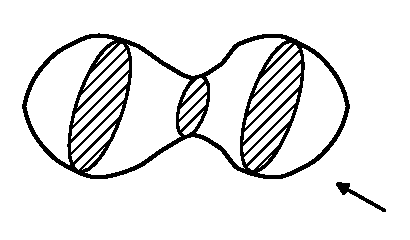
\includegraphics[width=5.2cm]{fig15.pdf}\\[0.3em]
{\small 图\ 15}
\end{minipage}\par

结果，我们得出热力学势振荡部分的最后公式
\begin{equation}
\left.\begin{aligned}
\widetilde{\Omega}&=\sum_{\mathrm{ex}}\sum_{l=1}^{\infty}(-1)^l\Omega_l
\cos\biggl\{\biggl(l\,\frac{\hbar^2S_{\mathrm{ex}}}{2m\beta B}\pm\frac{\pi}{4}\biggr)\biggr\},\\
\Omega_l&=\frac{2V(m\beta B)^{5/2}}{\pi^{7/2}\hbar^3m^*l^{5/2}}\,
\biggl|\frac{\partial^2S(\mu,k_z)}{\partial k_z^2}\biggr|_{\mathrm{ex}}^{-1/2}\,
\frac{\lambda}{\sinh\lambda}\,
\cos\biggl(\pi l\,\frac{m^*}{m}\,\xi_{\mathrm{ex}}\biggr),\\
\lambda&=l\pi^2Tm^*/m\beta B
\end{aligned}\right\}
\end{equation}
（$m$是电子的真实质量，余弦宗量的＋号或－号对应于极小截面或极大截面）.\footnote{自由电子气的费米面是半径为$k_{\mathrm F}=\sqrt{2m\mu}/\hbar$的球面，$S_{\mathrm{ex}}=\pi k_{\mathrm F}^2$，而公式(63.11)过渡到第五卷§60中的公式(60.15).}磁化强度$\bm{M}$（单位体积的磁矩）由微商算出\footnote{对$\bm B$的微商需要进行说明. 应用下面的方法能够得到公式(63.12). 当场的矢势作无限小的变化时，系统的哈密顿量的变化是
\begin{equation*}
\delta\hat H=\frac{1}{c}\int\hat{\bm j}\,\delta\bm A\,\mathrm dV,
\end{equation*}
其中$\hat{\bm j}$是流密度算符［参看第三卷(115.1)式］. 用$\delta\hat H$的平均值可以得到热力学势$\Omega$的变化（当$\mu,T,V$已给时）. 但是系统的量子化不是用精确的微观场$\bm H$（§62中已指出），而是用它的宏观平均值$\bm B$确定的. 就是说在$\delta\hat H$中也应该将$\bm A$理解成平均场$\bm B$的矢势. 于是，变分$\delta\bm A$可以从平均号下提出来，因而
\begin{equation*}
\delta\Omega=\langle\delta H\rangle=-\frac{1}{c}\int\langle\hat{\bm j}\rangle\,\delta\bm A\,\mathrm dV.
\end{equation*}
现在，根据定义$\langle\bm j\rangle=c\,\bm\nabla\times\bm M$引入磁矩，进行分部积分，我们得到
\begin{equation*}
\delta\Omega=-\delta\bm B\int\bm M\,\mathrm dV.
\end{equation*}}
\begin{equation}
\bm{M}=-\frac{1}{V}\,\frac{\partial\Omega}{\partial B}.
\end{equation}
这时，(63.11)式中要微商的只是变化最快的因子——余弦. 由于费米面的各向异性（$m^*$和$S_{\mathrm{ex}}$与场方向有关），一般说来，$\bm{M}$的方向与$\bm{B}$的不相重合. 我们得出纵向（沿场方向）磁化强度的振荡部分：
\begin{equation}
\begin{aligned}
\widetilde{M}_z&=\sum_{\mathrm{ex}}\sum_{l=1}^{\infty}(-1)^{l+1}M_l
\sin\biggl\{\biggl(l\,\frac{\hbar^2S_{\mathrm{ex}}}{2m\beta B}\pm\frac{\pi}{4}\biggr)\biggr\},\\
M_l&=\frac{B^{1/2}(m\beta)^{3/2}S_{\mathrm{ex}}}{\pi^{7/2}m^*l^{3/2}\hbar}\,
\biggl|\frac{\partial^2S(\mu,k_z)}{\partial k_z^2}\biggr|_{\mathrm{ex}}^{-1/2}\,
\frac{\lambda}{\sinh\lambda}\,
\cos\biggl(\pi l\,\frac{m^*}{m}\,\xi_{\mathrm{ex}}\biggr).
\end{aligned}
\end{equation}
表达式(63.11)和(63.13)是磁场的复杂振荡函数，并且一般说来，这些函数包含各种周期的项：来自费米面的每个极值截面的项都有一个关于变量$1/B$的周期，它等于
\begin{equation}
\Delta\,\frac{1}{B}=\frac{4\pi m\beta}{\hbar^2S_{\mathrm{ex}}}
=\frac{2\pi|e|}{c\hbar S_{\mathrm{ex}}}.
\end{equation}
我们注意到，这些周期都与温度无关.

振幅与温度的关系由因子$\lambda/\sinh\lambda$来确定. 当$\lambda\gg1$时，振幅按指数衰减，实际上振荡消失. 当$\lambda\lesssim1$时，因子$\lambda/\sinh\lambda\sim1$，因此振幅的数量级由$\Omega_l$和$M_l$中其余的因子来确定，下面的所有估算都属于这种情况.

为了粗略的估计，我们取
\begin{equation*}
m^*\sim m,\qquad \mu\sim\hbar^2k^2_{\mathrm F}/m,\qquad S\sim k^2_{\mathrm F}
\end{equation*}
其中$k_{\mathrm F}\sim1/a$，是费米面的线度. 于是得出
\begin{equation}
\widetilde{\Omega}\sim V\,\frac{(m\beta B)^{5/2}}{\hbar^3}
\sim Vn\mu\Bigl(\frac{\beta B}{\mu}\Bigr)^{5/2},\qquad
\widetilde{\bm{M}}\sim n\beta\Bigl(\frac{\beta B}{\mu}\Bigr)^{1/2}.
\end{equation}
其中$n\sim k^3_{\mathrm F}$是电子数密度. 当涉及磁化强度与场是单调关系的那部分（以$\overline{\bm{M}}$标记），可以进行估算，这只要取
\begin{equation}
\overline{\bm{M}}\sim\bar{\chi}\,\bm{B}\sim\beta^2\,\frac{mk_{\mathrm F}}{\hbar^2}\,\bm{B}
\sim n\beta\,\frac{\beta B}{\mu}.
\end{equation}
其中$\bar{\chi}$是磁化率的“单调”部分，比如按照电子气在弱场中的磁化率公式（参看第五卷§59）估算. 相应的热力学势的单调部分是
$\overline{\Omega}\sim V\overline{\bm{M}}\bm{B}\sim Vn\mu(\beta B/\mu)^2$. 对比所写出的表达式，表明热力学势的振荡部分小于它的磁性单调部分：
\begin{equation*}
\widetilde{\Omega}/\overline{\Omega}\sim(\beta B/\mu)^{1/2}\ll1.
\end{equation*}
尤其小于它在无磁场时的值$\Omega_0\sim Vn\mu$：$\widetilde{\Omega}/\Omega_0\sim(\beta B/\mu)^{5/2}$. 相反地，磁化强度的振荡部分远大于其单调部分
\begin{equation*}
\widetilde{\bm{M}}/\overline{\bm{M}}\sim(\mu/\beta B)^{1/2}\gg1.
\end{equation*}
应该指出，所有上述磁化振荡的理论是关于理想晶体电子液体的，在理论中未考虑传导电子在声子和在晶格缺陷（如杂质原子）上的散射过程可能带来的影响. 这些过程导致电子能量的不确定性：$\Delta\varepsilon\sim\hbar/\tau\sim\hbar v_{\mathrm F}/l$（其中$\tau$是两次碰撞间隔的时间；$l$是自由程；$v_{\mathrm F}$是电子速度）. 细锐能级的弥散也导致磁化振荡的平滑化. 允许忽略散射过程的条件在于能量的不确定值$\Delta\varepsilon$小于能级间隔，也就是说，必须有：
\begin{equation}
\hbar\omega_B\gg\hbar v_{\mathrm F}l.
\end{equation}
在$T\to0$时（条件(63.1)）允许有任意小的$B$值［确切地说只是条件(63.17)所限定之值］. 此时磁化强度$\widetilde{\bm{M}}$，原则上可以同磁感应强度$\bm{B}$相比较［因为$\widetilde{M}/B\sim\bar{\chi}(\mu/\beta B)^{1/2}$］，但是，磁化率$\chi=\delta M/\delta H$\footnote{为了避免不必要的繁杂，以后当定性讨论所出现的效应时，我们不考虑各向异性的影响.}早已变大（对其模来说）. 实际上，还要指出，应该微商的只是振荡因子，于是得出
\begin{equation}
|\bar{\chi}|\sim\bar{\chi}\,(\mu/\beta B)^{3/2}.
\end{equation}
在这样情况下，磁化强度的振荡使宏观场强$\bm{H}=\bm{B}-4\pi\bm{M}(\bm{B})$与磁感应强度$\bm{B}$的关系曲线相继出现一系列的弯曲，有如图16所示（A.\,B.\,Pippard, 1963）. 但是，热力学稳定性条件要求\footnote{对比第Ⅷ卷§18，在那里对于电学导出类似的条件.}
\begin{equation*}
\Bigl(\frac{\partial H}{\partial B}\Bigr)_{T,\mu}>0.
\end{equation*}
因此与$bc$段曲线对应的状态是不可能的. 这里出现的情况与压强对体积的曲线关系上出现折弯时使物质产生相变（比较第五卷§84，§152）有完全类似的地方. $H(\bm{B})$的平衡曲线实际上对应于水平的直线线段$ad$，它使图上的两部分阴影面积相等；$ab$段和$cd$段则对应于亚稳态.

\par\nopagebreak\noindent\begin{minipage}{\linewidth}\centering
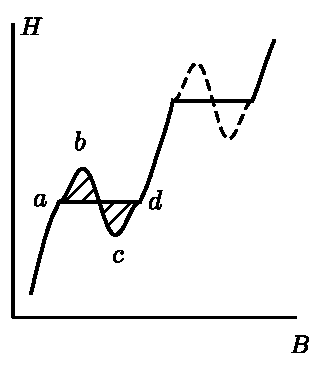
\includegraphics[width=4.6cm]{fig16.pdf}\\[0.3em]
{\small 图\ 16}
\end{minipage}\par

假如金属样品是圆柱体的，它的轴与外场$\mathfrak{H}$同方向. 这时，圆柱体内的磁场强度$H$同$\mathfrak{H}$相等，并且随着$\mathfrak{H}$的增大，物体将经历一系列的相变，此时磁感应强度有阶跃式的变化：每次当达到例如$a$点时，磁感应强度突然地由$B_a$变到$B_d$\footnote{各相之间分界面的表面能假定为正.}. 如果样品是与磁场垂直的平薄板，则物体将被分割为一些具有不同磁感应强度的交替层（\textbf{抗磁畴}）. 这完全类似于将中间态的超导体分为正常层和超导层（J.\,H.\,Condon, 1966）. 这时，外场$\mathfrak{H}$等于磁感应强度对各层的平均值. 例如，在区间$B_a<\mathfrak{H}<B_d$，薄板分成磁感应强度为$B_a$和$B_d$两层，随着$\mathfrak{H}$的增加，$B_d$层的体积增加，而$B_a$层的体积则相应减少.

\section{电子-声子相互作用}

迄今为止，我们研究晶格中的传导电子，都未涉及它同晶格振动（即声子）的相互作用. 这个相互作用表明如下的事实，晶格的形变改变了场，而电子在这个场中运动；场的这个变化称为\textbf{形变势}.

电子－声子的相互作用在半导体和金属的动理学现象中起决定性的作用，但是在这里，我们感兴趣的只是这个相互作用对电子能谱定性的影响. 为了研究相互作用，最好避开与晶格的各向异性以及与微观非均匀性有关的复杂情况. 换句话说，我们所研究的介质是看作微观均匀的各向同性的液体，与此对应的，在介质中只能发生纵向声振动.

对于形变的一级近似，这个简化模型的形变势表成下式
\begin{equation}
U_{\text{形变}}(\bm{r})=\frac{1}{\rho}\int
W(\bm{r}-\bm{r}')\rho'(\bm{r}')\,\mathrm{d}^3x',
\end{equation}
其中$\rho'$是介质密度的变化部分（而$\rho$是恒定的平衡值）. 函数$W(\bm{r}-\bm{r}')$在数量级为原子间距$a$的长度上要减小. 我们进一步简化(64.1)式，注意到，同波矢为$\bm{k}\ll1/a$的声子作用时，此距离可以认为等于零. 即取$W=w\,\delta(\bm{r}-\bm{r}')$，其中$w$是常数，则$U_{\text{形变}}=w\cdot\rho'(\bm{r})/\rho$. 在量子理论二次量子化表象里，这个势作为电子－声子相互作用的哈密顿量可写成
\begin{equation}
\hat{H}_{\text{电声}}=\frac{w}{\rho}\int
\hat{\varPsi}^{+}_\alpha(t,\bm{r})\,\hat{\rho}'(t,\bm{r})\,
\hat{\varPsi}_\alpha(t,\bm{r})\,\mathrm{d}^3x,
\end{equation}
其中$\hat{\varPsi},\hat{\varPsi}^{+}$是电子算符，而$\hat{\rho}'$是描写声子场的海森伯密度算符；对于自由（同电子无作用）的声子，此算符由(24.10)式给出.

在格林函数的数学工具中，用于电子－声子相互作用的，除了电子格林函数$G$外，还有如下定义的声子格林函数
\begin{equation}
D(X_1,X_2)\equiv D(X_1-X_2)
=-\mathrm{i}\langle T\hat{\rho}'(X_1)\hat{\rho}'(X_2)\rangle.
\end{equation}
此时，编时乘积按玻色子情形的规则(31.2)来展开. 对于自由声子，在动量表象中的格林函数是
\begin{equation}
D^{(0)}(\omega,\bm{k})=\frac{\rho k}{2u}
\biggl\{\frac{1}{\omega-uk+\mathrm{i}0}
-\frac{1}{\omega+uk-\mathrm{i}0}\biggr\}
=\frac{\rho k^2}{\omega^2-u^2k^2+\mathrm{i}0}
\end{equation}
（参阅§31中的习题；在中间的公式里取$\hbar=1$）.

我们把电子－声子相互作用看成微扰，可以根据算符(64.2)来建立图技术. 这同§13中对费米子配对相互作用所做过的一样，不再重复全部的讨论，而叙述所得到的（在动量表象中的）作图规则\footnote{电子－声子相互作用算符的表达式(64.2)的构造类似于量子电动力学中的电子——光子相互作用算符的构造，因此，两种情况的图技术规则也相似.}.

图的基本元素是电子线（实线）和声子线（虚线）. 每一条线都用一定的“4－动量”来描述. 4－动量为$P$的电子线对应于因子$\mathrm{i}G^{(0)}_{\alpha\beta}=\mathrm{i}\delta_{\alpha\beta}G^{(0)}(P)$，即自由电子格林函数. 4－动量为$K$的声子线对应于因子$\mathrm{i}D^{(0)}(K)$，即自由声子格林函数. 图的每个顶点会聚两条实线和一条虚线；每个顶点还有一个附加因子$-\mathrm{i}w/\rho$.

例如，电子格林函数的第一级修正用下图描绘\footnote{由于$D^{(0)}(0)=0$而不存在自封闭电子线的图［类似图(13.13a)］. 这里意味着，在$\omega\to0$之前即已过渡到极限$\bm k\to0$. 这反映如下的事实：在哈密顿量的定义(64.2)中，已经包含坐标空间内对$\mathrm d^3x$的积分（此时刚好表示过渡到$\bm k\to0$），因此，这个积分在对时间积分之前便完成了. 在哈密顿量中应用微扰论时便出现这个对时间的积分.}
\begin{equation}
\setlength{\unitlength}{1pt}%
\begin{picture}(205,80)(0,2)
  % ---- 左外线（实线，箭头向左） ----
  \put(70,40){\line(-1,0){28}}
  \put(42,40){\vector(-1,0){30}}
  \put(14,30){\makebox(0,0){$P$}}
  % ---- 右外线（实线，箭头向左） ----
  \put(130,40){\line(1,0){28}}
  \put(158,40){\vector(-1,0){28}}
  \put(190,30){\makebox(0,0){$P$}}
  % ---- 上弧：声子线 K（虚线，箭头指向左顶点） ----
  \qbezier(70.0,40.0)(71.5,42.2)(73.0,44.2)
  \qbezier(75.5,47.3)(77.0,49.1)(78.5,50.7)
  \qbezier(80.9,53.1)(82.4,54.5)(83.9,55.7)
  \qbezier(86.4,57.5)(87.9,58.5)(89.4,59.2)
  \qbezier(91.8,60.4)(93.3,61.0)(94.8,61.3)
  \qbezier(97.3,61.8)(98.8,62.0)(100.3,62.0)
  \qbezier(102.7,61.8)(104.2,61.6)(105.7,61.2)
  \qbezier(108.2,60.4)(109.7,59.8)(111.2,58.9)
  \qbezier(113.6,57.5)(115.1,56.5)(116.6,55.2)
  \qbezier(119.1,53.1)(120.6,51.7)(122.1,50.1)
  \qbezier(124.5,47.3)(126.0,45.5)(127.5,43.5)
  \put(82.0,54.1){\vector(-1,-1){9}}
  \put(100,70){\makebox(0,0){$K$}}
  % ---- 下弧：电子线 P−K（实线，箭头指向左顶点） ----
  \qbezier(70,40)(100,-4)(130,40)
  \put(82.0,25.9){\vector(-1,1){9}}
  \put(100,12){\makebox(0,0){$P-K$}}
\end{picture}
\end{equation}
其对应的解析式为
\begin{equation}
\mathrm{i}\delta G(P)=-\frac{w^2}{\rho^2}\,[G^{(0)}(P)]^2
\int G^{(0)}(P-K)D^{(0)}(K)\,\frac{\mathrm{d}^4K}{(2\pi)^4},
\end{equation}
声子格林函数的第一级修正用下图描述
\begin{equation}
\setlength{\unitlength}{1pt}%
\begin{picture}(205,80)(0,2)
  % ---- 左外线：声子线 K（虚线，箭头向左） ----
  \multiput(48,40)(4,0){6}{\line(1,0){2}}
  \put(46,40){\vector(-1,0){30}}
  \put(16,30){\makebox(0,0){$K$}}
  % ---- 右外线：声子线 K（虚线，箭头向左） ----
  \multiput(134,40)(4,0){6}{\line(1,0){2}}
  \multiput(162,40)(4,0){6}{\line(1,0){2}}
  \put(160,40){\vector(-1,0){26}}
  \put(188,30){\makebox(0,0){$K$}}
  % ---- 上弧：电子线 P（实线，箭头指向左顶点） ----
  \qbezier(70,40)(100,84)(130,40)
  \put(82.0,54.1){\vector(-1,-1){9}}
  \put(100,70){\makebox(0,0){$P$}}
  % ---- 下弧：电子线 P−K（实线，箭头指向右顶点） ----
  \qbezier(70,40)(100,-4)(130,40)
  \put(118.0,25.9){\vector(1,1){9}}
  \put(100,12){\makebox(0,0){$P-K$}}
\end{picture}
\end{equation}
其解析式则为
\begin{equation}
\mathrm{i}\delta D(K)=2\,\frac{w^2}{\rho^2}\,[D^{(0)}(K)]^2
\int G^{(0)}(P)G^{(0)}(P-K)\,\frac{\mathrm{d}^4P}{(2\pi)^4}
\end{equation}
（系数2产生于自旋因子的缩并：$\delta_{\alpha\beta}\delta_{\beta\alpha}=2$；与存在一个闭合费米子圈相应也要计及因子$-1$，比较§13）.

我们来证明，金属中电子－声子的相互作用在费米面附近将导致电子间“有效引力”的出现. 这可以直观地描绘成一个电子放出虚声子而被另一个电子所吸收（J.\,Bardeen, 1950; H.\,Fr\"{o}hlich, 1950\mbox{）.}

我们研究两个电子交换虚声子而实现散射的图：
\begin{equation}
\setlength{\unitlength}{1pt}%
\begin{picture}(190,158)(0,0)
  % ---- 上顶点两腿 ----
  \put(92,102){\vector(-3,4){46}}
  \put(56,146){\makebox(0,0){\small$P'_1=P_1+K$}}
  \put(130,138){\vector(-1,-1){36}}
  \put(138,146){\makebox(0,0){\small$P_1$}}
  % ---- 中间声子虚线 K（箭头向上） ----
  \multiput(92,58)(0,4){8}{\line(0,1){2}}
  \put(92,86){\vector(0,1){14}}
  \put(102,76){\makebox(0,0){\small$K$}}
  % ---- 下顶点两腿 ----
  \put(128,18){\vector(-1,1){36}}
  \put(138,12){\makebox(0,0){\small$P_2$}}
  \put(92,52){\vector(-3,-4){46}}
  \put(56,6){\makebox(0,0){\small$P'_2=P_2-K$}}
\end{picture}
\end{equation}
4－动量$P=(\varepsilon-\mu,\bm{p})$，$K=(\omega,\bm{k})$，$\mu$是$T=0$时电子的化学势，它等于界面能量$\varepsilon_{\mathrm F}$. 与此图对应的顶角函数为
\begin{equation*}
\Gamma_{\gamma\delta,\alpha\beta}=\Gamma\delta_{\alpha\gamma}\delta_{\beta\delta},
\qquad
\mathrm{i}\Gamma=\Bigl(-\frac{\mathrm{i}w}{\rho}\Bigr)^{\!2}\mathrm{i}D^{(0)}(K),
\end{equation*}
或
\begin{equation}
\Gamma=-\frac{w^2k^2}{\rho(\omega^2-u^2k^2+\mathrm{i}0)}
\end{equation}
此时$\hbar\omega=\varepsilon'_1-\varepsilon_1$，$\hbar\bm{k}=\bm{p}'_1-\bm{p}_1$.

按数量级，费米面附近电子的动量$p\sim p_{\mathrm F}\sim\hbar/a$. 声子动量$\hbar k\sim\hbar/a$和能量$\hbar uk\sim\hbar u/a\sim\hbar\omega_{\mathrm D}$对应于电子的散射角$\sim1$，其中$\omega_{\mathrm D}$是德拜频率（对于金属$\hbar\omega_{\mathrm D}\ll\varepsilon_{\mathrm F}$）. 另一方面，电子不能给出比$\varepsilon-\varepsilon_{\mathrm F}$还大的能量. 因此，如果对于两个电子都有$|\varepsilon-\varepsilon_{\mathrm F}|\ll\omega_{\mathrm D}$，则显然有
\begin{equation}
\Gamma\approx w^2/\rho u^2>0.
\end{equation}
考虑到$\Gamma$的意义是散射幅（§16），我们见到，它的符号对应于粒子间有引力. 要强调指出，这个结果只适于动量空间费米面附近薄层（其宽度按能量来说$\sim\hbar\omega_{\mathrm D}$）内的电子. 在金属超导理论中确定截断参数的大小时在§43中已经利用过这个情况\footnote{当谈到常数$w$时，为了粗略估计金属的$w$，可以指出，电子能量的变化应该达到它本身的数量级（$\sim\varepsilon_{\mathrm F}$），于是密度的变化$\rho'\sim\rho$. 因此$w\sim\varepsilon_{\mathrm F}$.}.

\section{电子-声子相互作用对金属中电子能谱的影响}

现在我们研究电子－声子相互作用对金属中电子能谱影响的问题\footnote{这一节所叙述的结果属于А.\,Б.\,Мигдал的工作（1958）.}.

在§14中已证明，对费米型能谱色散律$\varepsilon(\bm{p})$的修正（与自由费米系对比），由下列差式决定
\begin{equation}
\delta\varepsilon(\bm{p})=\Sigma(\varepsilon-\mu,\bm{p})-\Sigma(0,\bm{p}),
\end{equation}
其中$\Sigma=G^{(0)-1}-\varepsilon^{-1}$是自能函数. 在这种情况下所说的是与声子相互作用引起的修正，而各个粒子（电子）“直接”作用是谱的“非微扰”部分. 根据(64.6)式，有\footnote{在中间的公式中取$\hbar=1$.}
\begin{equation}
\begin{aligned}
\Sigma(P)&=-\delta G^{-1}=\delta G/[\,G^{(0)}\,]^2={}&\\
&=\mathrm{i}\,\frac{w^2}{\rho^2}\int G^{(0)}(P-K)D^{(0)}(K)\,
\frac{\mathrm{d}^4K}{(2\pi)^4}
\end{aligned}
\end{equation}
但是现在应该把$G^{(0)}$理解为电子间彼此相互作用的格林函数. 在其极点附近这个函数为
\begin{equation}
G^{(0)}(\varepsilon-\mu,\bm{p})=
Z\bigl[\varepsilon-\mu-v^{(0)}_{\mathrm F}(\bm{p}-\bm{p}_{\mathrm F})
+\mathrm{i}0\cdot\mathrm{sign}(\varepsilon-\mu)\bigr]^{-1}
\end{equation}
［参阅(10.2)式］；$v_{\mathrm F}$的上标(0)表明这个量还没计及电子－声子相互作用的影响.

现在，我们的目的是估算量值(65.1)，即积分
\begin{equation}
\begin{aligned}
\delta\varepsilon=\frac{\mathrm{i}w^2}{\rho^2}\int
\bigl\{G^{(0)}(\varepsilon-\mu-\omega,\bm{p}-\bm{k})
-G^{(0)}(-\omega,\bm{p}-\bm{k})\bigr\}\,\cdot{}\\
\cdot\,D^{(0)}(\omega,\bm{k})\,\frac{\mathrm{d}^4K}{(2\pi)^4}
\end{aligned}
\end{equation}
由下面的计算可以看到，对这个积分起主导作用的是来自动量$\bm{p}-\bm{k}$和能量$\varepsilon-\omega$靠近费米面附近的区域（$p$和$\varepsilon$的本身也是这样），即$\bm{k}\ll\bm{p}_{\mathrm F}$，$\omega\ll\mu$. 根据这个原因，函数$G^{(0)}$可以使用(65.3)式.

在$\bm{k}$空间内，沿$\bm{p}$方向取极轴的球坐标系中，我们有
$\mathrm{d}^4K=2\pi k^2\,\mathrm{d}k\,\mathrm{d}\omega\,\mathrm{d}\cos\theta$，其中$\theta$是$\bm{k}$和$\bm{p}$的夹角. 引进变量$p_1=|\bm{p}-\bm{k}|$替代$\cos\theta$；注意到$p_1^2=p^2+k^2-2pk\cos\theta$，我们有
\begin{equation*}
\mathrm{d}^4K=2\pi k^2\,\mathrm{d}k\,\mathrm{d}\omega\,
p_1\,\mathrm{d}p_1/pk\approx2\pi k\,\mathrm{d}k\,\mathrm{d}\omega\,\mathrm{d}p_1
\end{equation*}
（取$p_1\approx p\approx p_{\mathrm F}$）.

在(65.4)的被积式中只是花括号的因子才与$p_1$有关系，花括号等于
\begin{equation*}
\begin{aligned}
\{\cdots\}&=-(\varepsilon-\mu)Z\bigl[\varepsilon-\mu-\omega
-v^{(0)}_{\mathrm F}(p_1-p_{\mathrm F})
+\mathrm{i}0\cdot\mathrm{sign}(\varepsilon-\mu-\omega)\bigr]^{-1}\\
&\qquad\times\bigl[-\omega-v^{(0)}_{\mathrm F}(p_1-p_{\mathrm F})
-\mathrm{i}0\cdot\mathrm{sign}\ \omega\bigr]^{-1}.
\end{aligned}
\end{equation*}
由于对$\mathrm{d}(p_1-p_{\mathrm F})$的积分迅速收敛，可以把积分扩展到$\pm\infty$；引入变量$\eta=v^{(0)}_{\mathrm F}(p_1-p_{\mathrm F})$，我们得到积分
\begin{equation*}
\begin{aligned}
\int\{\cdots\}\,\mathrm{d}p_1&=-\frac{(\varepsilon-\mu)Z}{v^{(0)}_{\mathrm F}}\times{}\\
&\times\int_{-\infty}^{\infty}
\frac{\mathrm{d}\eta}{\bigl[\eta-(\varepsilon-\mu-\omega)
-\mathrm{i}0\cdot\mathrm{sign}(\varepsilon-\mu-\omega)\bigr]
\bigl[\eta+\omega+\mathrm{i}0\cdot\mathrm{sign}\ \omega\bigr]}.
\end{aligned}
\end{equation*}
如果被积式中的两个极点处在实轴的同一侧，那么积分等于零（使积分围道在另一半面上封闭，就会相信这一点）. 因此，仅当$\varepsilon-\mu>\omega>0$或者$\varepsilon-\mu<\omega<0$时积分才不等零，在第一种情况积分值为$-2\pi\mathrm{i}Z/v^{(0)}_{\mathrm F}$，第二种情况为$2\pi\mathrm{i}Z/v^{(0)}_{\mathrm F}$. 再考虑$D^{(0)}(\omega,\bm{k})$对变量$\omega$是偶函数，于是得到
\begin{equation}
\delta\varepsilon=\frac{Zw^2}{8\pi^2\rho uv^{(0)}_{\mathrm F}}
\int\limits_0^{|\varepsilon-\mu|}
\biggl[\frac{1}{\omega-uk+\mathrm{i}0}
-\frac{1}{\omega+uk-\mathrm{i}0}\biggr]k^2\,\mathrm{d}\omega\,\mathrm{d}k.
\end{equation}
表达式的实部和虚部分别对应于准粒子（传导电子）谱的修正和准粒子的衰减. 首先研究衰减.

按照规则(8.11)从(65.5)中分离出虚部，我们得到
\begin{equation}
-\mathrm{Im}\ \delta\varepsilon=\frac{Zw^2}{8\pi\rho uv^{(0)}_{\mathrm F}}
\int k^2\,\mathrm{d}k
\end{equation}
对$k$的积分是从0到$|\varepsilon-\mu|/u$的区域内进行的，(65.5)式的被积式的极点$\omega=uk$位于这个区域的0到$|\varepsilon-\mu|$的间隔内. 因此（在通常的单位制中）
\begin{equation}
-\mathrm{Im}\ \delta\varepsilon=
\frac{Zw^2|\varepsilon-\mu|^3}{24\pi\hbar^3\rho u^4v^{(0)}_{\mathrm F}}
\end{equation}
对这个量进行粗略估计，我们发现，参量$v^{(0)}_{\mathrm F}$和$w$起源于电子，因此在数量级上只通过原子间距$a$和电子质量$m$就可表达：
$v^{(0)}_{\mathrm F}\sim p_{\mathrm F}/m\sim\hbar/am$，
$\omega\sim\varepsilon_{\mathrm F}\sim\hbar^2/ma^2$（参阅273页的注解）. 密度$\rho$和声速$u$还与离子的质量$M$有关，并且$\rho\propto M$，$u\propto M^{-1/2}$，因而$\rho u^4\propto1/M$. 所以对衰减的估计可写成下式：
\begin{equation}
-\mathrm{Im}\ \delta\varepsilon\sim
|\varepsilon-\mu|^3\,(\hbar\omega_{\mathrm D})^{-2},
\end{equation}
其中德拜频率$\omega_{\mathrm D}\sim u/a\propto M^{-1/2}$.

严格说来，(65.8)式的估计与$|\varepsilon-\mu|\ll\hbar\omega_{\mathrm D}$相关，这时(65.6)式的积分按$k<|\varepsilon-\mu|/\hbar u\ll\omega_{\mathrm D}/u$范围进行. 这里实际利用了我们用过的声子色散律$\omega=ku$，但是，对于数量级的粗略估计甚至在$\varepsilon-\mu\sim\hbar\omega_{\mathrm D}$的区域边界处也可以使用(65.8)式，在这里估算给出
\begin{equation}
-\mathrm{Im}\ \delta\varepsilon\sim\hbar\omega_{\mathrm D}\sim|\varepsilon-\mu|.
\end{equation}
最后，当$\varepsilon-\mu\gg\hbar\omega_{\mathrm D}$时，(65.6)式的积分域与$\varepsilon-\mu$无关，因为极点$\omega=uk\lesssim\omega_{\mathrm D}$总是位于0到$\varepsilon-\mu$的间隔中. 在这种情况下
$\int k^2\mathrm{d}k\sim(\omega_{\mathrm D}/u)^3$，衰减为
\begin{equation}
-\mathrm{Im}\ \delta\varepsilon\sim\hbar\omega_{\mathrm D}\ll\varepsilon-\mu.
\end{equation}
表达式(65.8—65.10)确定一种与电子辐射声子有关的特有的衰减\footnote{在准粒子产生低频声子时，能量守恒由等式$(\partial\varepsilon/\partial\bm k)\,\delta\bm k=\bm v\,\delta\bm k=u\,\delta\bm k$来表达；它只在$v>u$时才成立. 在金属里，因为$v_{\mathrm F}\gg u$，此条件总能得到满足.}. 我们看到，当$|\varepsilon-\mu|\ll\hbar\omega_{\mathrm D}$时，在十分靠近费米面处，根据(65.8)式，衰减不大
（$|\mathrm{Im}(\varepsilon-\mu)|\ll|\varepsilon-\mu|$），致使传导电子这一准粒子概念有完全确切的意义. 而在$\varepsilon-\mu\sim\hbar\omega_{\mathrm D}$区域，准粒子的衰减便可与其本身的能量相比拟，谱要弥散而且在很大程度上谱将失去意义. 但是，在离费米面有更大的距离时，在$\varepsilon-\mu\gg\hbar\omega_{\mathrm D}$时（当然仍有$\varepsilon-\mu\ll\mu$），根据(65.10)式，衰减保持同样的绝对值，又变得比能量$\varepsilon-\mu$小，因此准粒子又获得确定的意义. 当然，除由传导电子产生的声子衰减外也总有电子与电子的碰撞而产生的衰减. 这个衰减是一切正常费米液体所特有的（§1），它正比于$(\varepsilon-\mu)^2$，其数量级为$(\varepsilon-\mu)^2/\mu$，就是说在理论应用的范围内总是小的.

现在我们估算对$\varepsilon$（即对能谱本身）的实部的修正.

在(65.5)式中对$\mathrm{d}\omega$积分的实部给出它的主值
\begin{equation*}
\begin{aligned}
\mathrm{Re}\int_0^{|\varepsilon-\mu|}D^{(0)}(\omega,\bm{k})\,\mathrm{d}\omega
&=\frac{\rho k}{2u}\,P\int_0^{|\varepsilon-\mu|}
\biggl\{\frac{1}{\omega-uk}-\frac{1}{\omega+uk}\biggr\}\mathrm{d}\omega=\\
&=\frac{\rho k}{2u}\ln\biggl|\frac{\varepsilon-\mu-uk}{\varepsilon-\mu+uk}\biggr|.
\end{aligned}
\end{equation*}
因此，对于$\mathrm{Re}\,\delta\varepsilon$我们有（通常单位）
\begin{equation}
\mathrm{Re}\,\delta\varepsilon=\frac{Z\omega^2}{8\pi^2\rho uv^{(0)}_{\mathrm F}}
\int k^2\ln\biggl|\frac{\varepsilon-\mu-\hbar uk}{\varepsilon-\mu+\hbar uk}\biggr|
\,\mathrm{d}k.
\end{equation}
在$\varepsilon-\mu\gg\hbar\omega_{\mathrm D}$时，被积表达式中的对数$\sim\hbar uk/(\varepsilon-\mu)$，因此整个积分估算为
$\hbar uk^3_{\max}/(\varepsilon-\mu)\sim\hbar u/a^3(\varepsilon-\mu)$. 还注意到，由于在(65.11)式的分母中存在因子$\rho$，整个表达式$\propto1/M$，得出估算
\begin{equation*}
\mathrm{Re}\ \delta\varepsilon\sim(\hbar\omega_{\mathrm D})^2/(\varepsilon-\mu)
\ll\varepsilon-\mu.
\end{equation*}
于是，在这种情况下对谱的修正相当小，因此在费米面上以“无微扰”速度值$v^{(0)}_{\mathrm F}$给出谱的表达式：
\begin{equation}
\varepsilon-\mu\approx v^{(0)}_{\mathrm F}(\bm{p}-\bm{p}_{\mathrm F}),
\qquad \text{当}\ \varepsilon-\mu\gg\hbar\omega_{\mathrm D}.
\end{equation}
在$\varepsilon-\mu\ll\hbar\omega_{\mathrm D}$的区域，(65.11)式中的对数
$\sim(\varepsilon-\mu)/\hbar uk$，而积分的估算为
$(\varepsilon-\mu)k^2_{\max}/\hbar u\sim(\varepsilon-\mu)/\hbar ua^2$. 结果，整个表达式(65.11)与$\varepsilon-\mu$成正比，其系数与离子质量$M$无关（因乘积$\rho u^2$与$M$无关）. 这就是说，这个区域的谱的类型还是：
\begin{equation}
\varepsilon-\mu\approx v_{\mathrm F}(\bm{p}-\bm{p}_{\mathrm F}),
\qquad \text{当}\ \varepsilon-\mu\ll\hbar\omega_{\mathrm D}.
\end{equation}
但速度$v_{\mathrm F}$与$v^{(0)}_{\mathrm F}$的差别在数量级上同速度本身同大\footnote{当然，在这些条件下运用微扰论的一级近似，严格地说并不正确. 但是，考虑进一步的近似并不改变所得结果的性质：当第一级修正达到1的程度时，其余的修正也是这个程度.}.

因此，金属电子的费米型能谱用两个不同的速度值$v_{\mathrm F}$和$v^{(0)}_{\mathrm F}$来表征，一个用在费米面的极邻近处（$\varepsilon-\mu\ll\hbar\omega_{\mathrm D}$），而另一个用在$\varepsilon-\mu\gg\hbar\omega_{\mathrm D}$时. 低温（$T\ll\hbar\omega_{\mathrm D}$）金属的热力学性质由(65.13)式中的参量$v_{\mathrm F}$来表述. 对于频率$\omega\gg\omega_{\mathrm D}$时的金属光学性质一类的现象则由速度$v^{(0)}_{\mathrm F}$来确定.

\begin{xiti}
确定金属中由电子吸收所致的长波（$k\ll p_{\mathrm F}$）声子的衰减.

解：根据(64.8)式，对声子格林函数的修正由积分
\begin{equation*}
\begin{gathered}
\mathrm{i}\delta D^{-1}(\bm{K})=-\frac{2w^2}{\rho^2}
\int G^{(0)}(P)G^{(0)}(P-K)\,\frac{\mathrm{d}^4P}{(2\pi)^4},\\
P=(P_0,\bm{p}),\qquad K=(\omega,\bm{k})
\end{gathered}
\end{equation*}
给出. 但是，在$G$函数中还必须考虑与电子－短波声子相互作用有关的修正. 根据正文所述，这些修正只不过归之为用函数$G$替换$G^{(0)}$，不同于(65.3)的只是将速度$v^{(0)}_{\mathrm F}$换成$v_{\mathrm F}$，以及将重整化常数$Z$换成另一个$Z'$. 对于小$K$时的乘积$G^{(0)}(P)G^{(0)}(P-K)$可以利用公式(17.10). 对$\mathrm{d}p_0\,\mathrm{d}p$的积分归结为消除$\delta$函数，此后还留下对$\mathrm{d}\cos\theta$（$\theta$是$\bm{p}$和$\bm{k}$的夹角）的积分
\begin{equation*}
\delta D^{-1}(\omega,\bm{k})=-\frac{Z'^2w^2p^2_{\mathrm F}k}{2\pi^2\rho^2}
\int_{-1}^{1}\frac{\cos\theta\,\mathrm{d}\cos\theta}
{\omega-v_{\mathrm F}k\cos\theta+\mathrm{i}0}
\end{equation*}
（取$\omega>0$）. 极点$\cos\theta=\omega/kv_{\mathrm F}$位于积分区域内（因$v_{\mathrm F}>u$），而积分的虚部为
\begin{equation*}
\mathrm{Im}\,\delta D^{-1}=\frac{Z'^2w^2p^2_{\mathrm F}\omega}{2\pi\rho^2v^2_{\mathrm F}k},
\end{equation*}
声子色散律由方程$D^{(0)-1}+\delta D^{-1}=0$的根来确定，由此得到（在通常单位制中）
\begin{equation*}
\omega=uk(1-\mathrm{i}\alpha),\qquad
\alpha=\frac{Z'^2w^2p^2_{\mathrm F}}{4\pi\hbar^3\rho uv^2_{\mathrm F}}.
\end{equation*}
（我们对实部$\omega$的修正不感兴趣）. 乘积$\rho u\propto\sqrt{M}$，因此粗略估计时$\alpha\sim\sqrt{m/M}$，即衰减总是小的.
\end{xiti}

\section{固体电介质的电子谱}

非磁性电介质晶体的电子能谱的特性在于：第一激发能级距基态能级有一有限的距离；换句话说，基态能级和激发能谱之间存在能隙（对于一般电介质其数量级是几个电子伏）.

电介质晶体中的元激发可以直观地描述成原子的激发态，但是这个激发态不是属于任何确定的原子的. 晶格的平移对称性总要导致“集体”激发，这个集体激发在晶体内有如从一个原子跳往另一个原子进行传播. 与其它情况一样，这些激发可以认为是有确定能量和准动量的准粒子（此时称为\textbf{激子}）. 像所有准粒子一样，这些激子是一个一个出现的，激子具有整数角动量，因而遵守玻色统计\footnote{关于激子的概念是Я.\,И.\,Френкель（1931）首先引进的.}.

在准动量$\bm{k}$一定时，激子的能量可以取遍一系列不同的离散值$\varepsilon_s(\bm{k})$. 当准动量在一个倒格胞中取值时，每个函数$\varepsilon_s(\bm{k})$要在激子的某个\textbf{能带}中取值；不同的能带可以部分地交叠. 每个函数$\varepsilon_s(\bm{k})$的最小值都不等于零.

除激子以外，电介质中还存在其它类型的电子激发. 可以认为它们来自单个原子的电离结果. 每次这样的电离在电介质中都要导致两个独立传播的准粒子，即传导电子和“空穴”的出现. 空穴就是在原子中缺少一个电子，因此它的行为有如带正电的粒子. 这里讲到电子和空穴的运动，实际上我们指的是电介质电子的某种集体的激发态，与激子态相反，这些激发态伴有负的或正的元电荷的迁移.

电子和空穴具有半整数自旋，因而遵守费米统计. 但是，我们强调指出，电介质的电子－空穴谱绝没有金属费米型电子谱的特征. 此特征在于：在$\bm{k}$空间存在边界费米面，电子的准动量就位于边界费米面的附近. 在所考虑的情况根本不存在任何类似的面，因此同时出现的电子和空穴可以有任意的准动量.

仔细研究元激发的衰减，就可理解两种谱型之间更深刻的区别. 在费米液体中任何处在费米面之外的准粒子都能产生一对新的激发（粒子和空穴），因此这些准粒子也都具备有限的寿命. 当其离开费米面时，这寿命很快地减小（此外，金属中的电子还可辐射声子，参阅§65）. 在$T=0$时，理想晶格的电介质中，单个电子（或空穴）的衰减在能量最小值上方的有限间隔内严格等于零\footnote{当然，在有限温度时，总有因在其它准粒子上散射而引起的衰减.}. 事实上，在任何情况下的电子－空穴对的形成都需要有限的能量消耗（因为存在能隙$\Delta$，参阅下面内容）. 准粒子只有在它的速度$v$不小于声速$u$时才可能辐射声子（声学辐射）（参阅254页上的注释）.

传导电子和空穴的能量可能值$\varepsilon^{(e)}(\bm{k})$和$\varepsilon^{(h)}(\bm{k})$也占据能带. 在电介质中电子和空穴的能量最小可能值之和
$\Delta=\varepsilon^{(e)}_{\min}+\varepsilon^{(h)}_{\min}$通常称之为能隙宽度. 因为电子和空穴同时出现和消失，那么，不是单个的$\varepsilon^{(e)}_{\min}$和$\varepsilon^{(h)}_{\min}$值，而是这个和才具有实际意义；通常约定$\varepsilon^{(h)}_{\min}=0$. 无论准动量$\bm{k}=\bm{k}_0$是相同或是不同，电子和空穴的能量都可以达到最小值；准动量相同的情况称为\textbf{直接}能隙，而不同的情况称为间接能隙. 如果带中的能级不简并.（或者作为时间反演对称的结果，对自旋只有二重简并），那么函数在其极小值附近的形式是
\begin{equation}
\begin{gathered}
\varepsilon^{(e)}(\bm{k})=\Delta+\frac{1}{2}m^{(e)-1}_{ik}q_iq_k,\\
\varepsilon^{(h)}(\bm{k})=\frac{1}{2}m^{(h)-1}_{ik}q_iq_k,
\end{gathered}
\end{equation}
其中$\bm{q}=\bm{k}-\bm{k}_0$，而$m^{(e)}_{ik}$和$m^{(h)}_{ik}$是电子和空穴的有效质量张量.

在文献中电子能带常常简称之为\textbf{导带}，而代替空穴带的称之为\textbf{价带}，在晶体的基态，价带完全被电子填满. 这时，产生电子和空穴这一对准粒子，可以认为电子从价带跃迁到导带的结果，而在放弃的位置留下空穴.

在较大（同原子相比）的距离上，电子和空穴按库仑定律相互吸引. 因此它们能够形成束缚态. 被束缚的电子和空穴的总体是电中性准粒子，即激子. 在给定准动量时，电子＋空穴系统的离散能级对应于束缚态. 每条能级对应于激子的一个能带. 这样一来，激子能量便位于电子－空穴激发能的下面（因此，在本节初指出的能隙的含义与量$\Delta$不相一致，而是小于它，其差等于激子的最大束缚能）\footnote{但是因为电子和空穴能够复合而放出声子和光子，激子状态的寿命是有限的.}.

在弱束缚态这一极限情况下，电子和空穴之间的平均距离大于晶格常数$a$时，激子的能级便容易算得；这样的激子称为\textbf{瓦尼尔-莫特（Wannier-Mott）激子}. 在相反的极限情况，电子和空穴之间的距离为原子的数量级时，称为\textbf{弗仑克尔（Frenkel）激子}；当然，弗仑克尔激子只在形式上看成是电子和空穴的束缚态.

我们研究立方对称的电介质晶体. 对于瓦尼尔－莫特激子，可以认为电子和空穴是按库仑定律相互吸引的，而晶体中其余原子的作用只归结为均匀电介质背景，它使相互作用减小到$1/\varepsilon$，这里$\varepsilon$是晶体的电容率（对应于激子束缚能数量级的频率值）；换言之，电子与空穴的相互作用能写成$U=-e^2/\varepsilon r$的形式. 在能谱中设能隙是直接的，并且为了简单起见我们认为电子和空穴能量的最小值在$\bm{k}=0$处. 在立方晶体中有效质量张量归结为标量常数$m_e$和$m_h$，因此
\begin{equation}
\varepsilon^{(e)}(\bm{k})=\Delta+\frac{\hbar^2k^2}{2m_e},
\qquad
\varepsilon^{(h)}(\bm{k})=\frac{\hbar^2k^2}{2m_h}.
\end{equation}

在§56末已经指出，当晶格处于在空间缓慢变化的外电场时，用薛定谔方程来描述粒子在晶格内的运动，其哈密顿量中函数$\varepsilon(\bm{k})$起着动能的作用. 因为在这种情况下函数$\varepsilon^{(e)}(\bm{k})-\Delta$和$\varepsilon^{(h)}(\bm{k})$在形式上同通常的自由粒子的动能一致，于是我们所研究的系统的薛定谔方程在形式上便与按库仑相互作用的普通双粒子系统的薛定谔方程一致，即与氢原子问题的薛定谔方程一致. 因此，我们可以立刻写出系统的能级，即如下形式的激子能量
\begin{equation}
\varepsilon^{(\mathrm{ex})}_n(\bm{k})-\Delta
=\frac{\hbar^2k^2}{2(m_e+m_h)}
-\frac{me^4}{2\varepsilon^2\hbar^2n^2}
\end{equation}
（G.\,H.\,Wannier, 1937）. 这个表达式的第一项是激子以准动量$\bm{k}$作为“整体”运动的能量，第二项是激子中电子和空穴的束缚能［$m=m_em_h/(m_e+m_h)$是系统的折合质量］当$\bm{k}$已给时，随着能量向连续谱边界增大的同时，系统离散谱的能级便稠密起来. 公式(66.3)的适用条件是“轨道半径”值要充分大，即
$r_{\mathrm{ex}}\sim\hbar^2\varepsilon n^2/me^2\gg a$. 这个条件对于大$n$显然满足. 但是在大$\varepsilon$的晶体中对于$n\sim1$，此条件也满足\footnote{值得注意的是，能带上边缘（极大值）附近有效质量是负的，能够形成两个电子（或两个空穴）的束缚态. 这些态的能量位于禁戒区域内高于双电子总能量极大值的地方.}.

在本节最后，我们再谈谈§61中关于传导电子的数密度在半金属中存在下限的论断.

电介质中，在$T=0$时不存在电子和空穴，它们可能形成束缚态，这意味着只能出现能谱的新分支. 在补偿金属中这种可能性意味着：具有自由电子和自由空穴的态不是最低的态，即金属型能谱是不稳定的. 在电子和空穴之间存在别的准粒子而屏蔽库仑相互作用，这就消除了形成束缚态的可能性. 换句话说，准粒子间的平均距离必须与激子的线度$r_{\mathrm{ex}}$（在其基态）同数量级或者更小. 我们注意到，对于金属，由这个要求所建立的电子和空穴数密度的允许下限，随它们的有效质量之减小而下降.

\section{半导体中的电子和空穴}

纯净（或称\textbf{本征}）的半导体晶体的能谱与电介质能谱的区别仅在于量的方面，即前者能隙值$\Delta$较小，因此在通常温度下，半导体中存在相当大的（与电介质相比）载流子密度. 显然，这个差别是有条件的，并且也与我们所感兴趣的温度区域有关\footnote{我们写出某些半导体的能隙值$\Delta$：Si—1.17~eV，Ge—0.74~eV，InSb—0.24~eV，GeAs—1.52~eV，PbS—0.29~eV. 对于典型电介质金刚石$\Delta=5.4$~eV.}. 在\textbf{杂质}（或\textbf{合金}）半导体中杂质原子是电子或空穴的补充源，对于给晶格提供电子（\textbf{施主杂质}）或从晶格接受电子（\textbf{受主杂质}）的杂质原子，其能隙比基本谱的能隙小.

我们要详细讨论半导体（或电介质）中能隙大小$\Delta$与传导电子密度以及与空穴密度间的关系.

电子（e）和空穴（h）成对地产生和消失，从热力学观点看，可以当作“化学反应”$e+h\rightleftarrows0$（晶体的基态起“真空”作用）按普遍规则（参阅第五卷§101）这个反应的热力学平衡条件可写成下式
\begin{equation}
\mu_e+\mu_h=0,
\end{equation}
其中$\mu_e$和$\mu_h$是电子和空穴的化学势. 鉴于半导体中（在$T\ll\Delta$时）的电子密度（$n_e$）和空穴密度（$n_h$）都不算大，它们的费米分布可相当精确地归结为玻尔兹曼分布，因此电子和空穴形成经典气体\footnote{在常温下，半导体中电子和空穴的密度$10^{13}\sim10^{17}\,\mathrm{cm}^{-3}$，而在金属中它们的密度为$10^{22}\sim10^{23}\,\mathrm{cm}^{-3}$.}. 那么用通常的方式（见第五卷§101）根据条件(67.1)便得到质量作用定律，据此定律，平衡密度之积
\begin{equation}
n_en_h=K(T),
\end{equation}
式中的右方是只与基本晶格性质有关的温度函数. 在此晶格的原子上产生与湮灭电子和空穴；这个函数与是否有杂质无关. 我们计算函数$K(T)$，为了明确起见. 电子和空穴的能量采用准动量平方的函数(66.1).

单位体积内的电子按准动量的分布由玻尔兹曼分布给出
\begin{equation*}
\exp\biggl(\frac{\mu_e-\varepsilon_e(\bm{k})}{T}\biggr)
\,2\,\frac{\mathrm{d}^3k}{(2\pi)^3}
\end{equation*}
（因子2是考虑到自旋的两个取向）. 实行代换
\begin{equation*}
2\,\frac{\mathrm{d}^3k}{(2\pi)^3}\ \longrightarrow\
\frac{\sqrt{2}\,m^{3/2}_e}{\pi^2\hbar^3}\sqrt{\varepsilon_e-\Delta}\,
\mathrm{d}\varepsilon_e,
\end{equation*}
便过渡到按能量的分布，其中$m_e=(m_1m_2m_3)^{1/3}$，而$m_1,m_2,m_3$是有效质量张量$m^{(e)}_{ik}$的主值. 于是，单位体积的总电子数是
\begin{equation*}
n_e=\frac{\sqrt{2}\,m^{3/2}_e}{\pi^2\hbar^3}\,
\mathrm{e}^{\mu_e/T}\int_{\Delta}^{\infty}
\sqrt{\varepsilon_e-\Delta}\,\mathrm{e}^{-\varepsilon_e/T}\,\mathrm{d}\varepsilon_e
\end{equation*}
（鉴于快速收敛，积分可扩展到无穷大）. 计算积分，得出
\begin{equation}
n_e=2\biggl(\frac{m_eT}{2\pi\hbar^2}\biggr)^{3/2}
\mathrm{e}^{(\mu_e-\Delta)/T}.
\end{equation}
类似地，得到
\begin{equation}
n_h=2\biggl(\frac{m_hT}{2\pi\hbar^2}\biggr)^{3/2}\mathrm{e}^{\mu_h/T}.
\end{equation}
最后，把两个式子相乘且考虑到(67.1)式，获得所求的结果
\begin{equation}
n_en_h=\frac{(m_em_h)^{3/2}}{2\pi^3\hbar^6}\,T^3\,\mathrm{e}^{-\Delta/T}.
\end{equation}
在本征半导体中，全部电子和空穴都成对出现：
\begin{equation}
n_e=n_h=\frac{(m_em_h)^{3/4}}{\sqrt{2}\,\pi^{3/2}\hbar^3}\,
T^{3/2}\,\mathrm{e}^{-\Delta/2T}.
\end{equation}
取式(67.6)和式(67.3)相等，求得电子的化学势\footnote{在文献中这个量常常称为费米能级. 但是，我们着重指出，半导体中电子的化学势绝不具有在金属中才存在的界限能的含义.}
\begin{equation}
\mu_e=\frac{\Delta}{2}+\frac{3T}{4}\ln\frac{m_h}{m_e}.
\end{equation}
至于讲到电子和空穴对半导体热力学量的贡献，在$T\ll\Delta$时它是指数型微小. 考虑到产生一个电子－空穴对，需要接近$\Delta$的能量，电子－空穴给内能的贡献为$E_{eh}\approx Vn_e\Delta$，这里$n_e$取自(67.6)式. 这个量与晶格对晶体能量的贡献相比常可忽略不计.

\section{简并点附近的电子谱}

在这一节我们用简单的例子证明，如何从对称的考虑出发求出半导体（或电介质）中电子和空穴在$\bm{k}$空间（倒格子）某些特定点附近能谱的类型；这些特定点是按其对称性选出来的\footnote{不考虑电子的自旋时，这个问题在形式上与晶体中声子能谱的问题相同. 参阅第五卷§136.}.

我们研究的晶格属于立方晶类$O_h$，因而对$\bm{k}=0$点（即倒格子立方晶胞的顶点）附近的能谱感兴趣，这个点具有完全点群$O_h$的固有对称性.

作为第一个例子，我们研究不计电子自旋的能谱，并假定能带中的能级恰好在$\bm{k}=0$点上是二重简并的，并属于群$O_h$的不可约表示$E_g$\footnote{点群表示的记号见第三卷§95，§99.}. 离开$\bm{k}=0$点简并便消除；问题是寻求这一点附近的色散律$\varepsilon(\bm{k})$的全部分支.

在§59中说明过，在$\bm{k}$空间怎样才能把对某个$\bm{k}=\bm{k}_0$点的偏离当成微扰. 微扰算符的具体形式在这里对于我们是无紧要的. 只要知道每一级小量$\bm{q}=\bm{k}-\bm{k}_0$（在本情况下$\bm{k}_0=0$，因之$\bm{q}\equiv\bm{k}$）对能量修正式的结构就够了. 第一级修正项由$\bm{k}\cdot\hat{\bm{\gamma}}$型算符的矩阵元（对应于同一简并能级各状态之间的跃迁）构成的久期方程来确定，其中$\hat{\bm{\gamma}}$是某个矢量算符. 在本情况下，由于在对称群内存在反演中心，算符$\hat{\bm{\gamma}}$所有的矩阵元显然为零，因此不存在$\bm{k}$的一级效应（对比第五卷§136），对能量按$\bm{k}$的二级修正由下列算符的矩阵元所组成的久期方程来确定
\begin{equation}
\hat{V}=\hat{\bm{\gamma}}_{ik}k_ik_k
\end{equation}
这里$\hat{\bm{\gamma}}_{ik}$是某个厄米算符的张量（对$i,k$下标对称）；其中包含哈密顿量在微扰二级近似中的$\bm{k}$的线性修正项，也包含一级近似中的$\bm{k}$的二次修正项. 在算符(68.1)的矩阵元中显然有不为零的. 但是，由于对称性的要求，矩阵元之间有一定的关系.

在对称操作时，就其变换规律来说，作为表示$E_g$基底的波函数可以选取
\begin{equation*}
\psi_1\sim x^2+\omega y^2+\omega^2z^2,\qquad
\psi_2\sim x^2+\omega^2y^2+\omega z
\end{equation*}
的形式，其中
\begin{equation*}
\omega=\mathrm{e}^{2\pi\mathrm{i}/3},\qquad
\omega^2=\omega^*,\qquad 1+\omega+\omega^2=0.
\end{equation*}
在这里符号$\sim$代表“变换如”的意思. 绕立方的空间对角线转动$C_3$，使坐标按照$x,y,z\to z,x,y$变换；此时，函数$\psi_1,\psi_2$进行如下变换
\begin{equation*}
C_3\colon \psi_1\to\omega\psi_1,\qquad \psi_2\to\omega^2\psi_2,
\end{equation*}
绕立方体棱的转动$C^x_4$（$x,y,z\to x,-z,y$的变换）函数按照
\begin{equation*}
C^x_4\colon \psi_1\to\psi_2,\qquad \psi_2\to\psi_1
\end{equation*}
变换，等等. 在坐标反演时，$x,y,z$改变符号，而函数$\psi_1,\psi_2$不变.

由此容易得出，非对角分量$\hat{\bm{\gamma}}_{ik}$的所有矩阵元都为零，而对角分量的矩阵元归结为两个独立的实常数：
\begin{equation*}
\langle1|\gamma_{xx}|1\rangle=\langle2|\gamma_{xx}|2\rangle
=\langle1|\gamma_{yy}|1\rangle=\cdots\equiv A.
\end{equation*}
\begin{equation*}
\langle1|\gamma_{xx}|2\rangle=\langle2|\gamma_{xx}|1\rangle\equiv B,\quad
\langle1|\gamma_{yy}|2\rangle=\omega B.\quad
\langle1|\gamma_{zz}|2\rangle=\omega^2B,
\end{equation*}
现在算符(68.1)的矩阵元为
\begin{equation*}
\begin{gathered}
\langle1|V|1\rangle=\langle2|V|2\rangle=Ak^2,\\
\langle1|V|2\rangle=\langle2|V|1\rangle^{*}
=B\bigl(k_x^2+\omega k_y^2+\omega^2k_z^2\bigr).
\end{gathered}
\end{equation*}
用这些矩阵元构成久期方程并求解，我们得到能谱的两个分支：
\begin{equation}
\varepsilon_{1,2}(\bm{k})-\varepsilon(0)=Ak^2\pm
B\bigl[k^4-3(k_x^2k_y^2+k_x^2k_z^2+k_y^2k_z^2)\bigr]^{1/2}.
\end{equation}
除立方体对角线（$k_x=k_y=k_z$）外，在一切方向上离开$\bm{k}=0$点，都可使简并消除\footnote{对于表示$E_u$（在$\bm k=0$点）也可得到与(68.2)相同的结果. 在该点附近色散律对于如下一些不同的表示总是相同的，这些表示的区别只在于乘上任意的一维群表示（在该情况下$E_u=E_g\times A_{1u}$）. 显然，在这些情况下在不同的基函数之间的跃迁矩阵元以同样的关系相互联系.}.

作为另一个例子，我们研究具有电子自旋的能谱；此时对称群的双值（旋量）表示与能级相对应. 假设在$\bm{k}=0$点，与群$O_h$的不可约表示$D'_u$（或$D'_g$）\footnote{对于金刚石、硅和锗的空穴能带底就有这种情况，这些物质有同一类型的晶格.}相对应，能级是四重简并的.

这样表示的基函数可以选择如角动量$j=3/2$的本征函数
$\psi^j_m\ (m=-j,\cdots,j)$一样变换的函数\footnote{在第三卷§99的习题中已证明全旋转群的不可约表示$D^{(3/2)}$对群$O$仍保持为不可约的，并与其表示$D'$一致.}. 这件事情，允许我们运用下述方法而使问题的求解大大简化（J.\,M.\,Luttinger, 1956）.

对于四维表示，算符(68.1)的矩阵是$4\times4$的，有16个元素. 所有这样的矩阵都可表为16个已知的线性无关的$4\times4$矩阵的线性组合. 作为这样的矩阵，我们选
\begin{equation*}
\hat{j}_x,\ \hat{j}^2_x,\ \{\hat{j}_x,\hat{j}_y\}_+,\ \hat{j}^3_x,\
\{\hat{j}_x,\hat{j}^2_y-\hat{j}^2_z\}_+,
\end{equation*}
并且循环置换指标$x,y,z$，这有15个矩阵，再一个矩阵为
$\{\hat{j}_x,\{\hat{j}_y,\hat{j}_z\}_+\}_+$（记号$\{\cdots\}_+$表示反对易）. 这里$\hat{j}_x,\hat{j}_y,\hat{j}_z$是角动量$j=3/2$的笛卡儿分量对四个函数$\psi^{3/2}_m$所取的矩阵. 另一方面，这样选择基函数时必须认为算符$\hat{j}_x,\hat{j}_y,\hat{j}_z$在转动和反射时作为轴矢量的分量进行变换. 这个事实允许将算符$\hat{V}$写成$k_x,k_y,k_z$的二次型，它由对群$O_h$所有变换都是不变的表达式构成：
\begin{equation}
\begin{aligned}
\hat{V}&=\beta_1\bm{k}^2+4\beta_2\bigl(k^2_x\hat{j}^2_x+k^2_y\hat{j}^2_y+k^2_z\hat{j}^2_z\bigr)+{}\\
&\qquad+\beta_3\bigl(k_xk_y\{\hat{j}_x,\hat{j}_y\}_+
+k_yk_z\{\hat{j}_y,\hat{j}_z\}_+
+k_xk_z\{\hat{j}_z,\hat{j}_x\}_+\bigr),
\end{aligned}
\end{equation}
其中$\beta_1,\beta_2,\beta_3$是实常数.

现在，算符(68.3)对于函数
\begin{equation*}
\psi_1\sim\psi^{3/2}_{3/2},\quad
\psi_2\sim\psi^{3/2}_{1/2},\quad
\psi_3\sim\psi^{3/2}_{-1/2},\quad
\psi_4\sim\psi^{3/2}_{-3/2}
\end{equation*}
的矩阵元，根据熟知的角动量矩阵元［由第三卷公式(29.7—29.10)给出］容易算出. 这样的计算得出下面的表达式
\begin{equation}
\left.\begin{aligned}
V_{11}&=V_{44}=(\beta_1+3\beta_2)(k^2_x+k^2_y)+(\beta_1+9\beta_2)k^2_z,\\
V_{22}&=V_{33}=(\beta_1+7\beta_2)(k^2_x+k^2_y)+(\beta_1+\beta_2)k^2_z,\\
V_{12}&=-V_{34}=\frac{\sqrt{3}}{2}\,\beta_3k_x(k_y+\mathrm{i}k_x),\\
V_{13}&=V_{24}=2\sqrt{3}\,\beta_2(k^2_y-k^2_x)
+\frac{\sqrt{3}}{2}\,\beta_3\mathrm{i}k_xk_y,\\
V_{14}&=V_{23}=0.
\end{aligned}\right\}
\end{equation}
注意到能级显然不会完全分裂——还必须保留二重（克拉默斯型）简并，久期方程的构成就可以得到简化. 就是说，久期方程的每个根$\lambda\equiv\varepsilon(\bm{k})-\varepsilon(0)$（矩阵$\hat{V}$的本征值）将是重根. 换句话说，每个本征值$\lambda$将有两个线性无关的一组量$\varphi_n\ (n=1,2,3,4)$与之对应，它们是方程
\begin{equation}
\sum_nV_{nm}\varphi_m=\lambda\varphi_n
\end{equation}
的解. 于是叠加这两组量，我们可以给量$\varphi_n$附加一个补充条件，特别是使一个量为零，如取$\varphi_4=0$，则$n=4$的方程(68.5)给出
\begin{equation*}
V_{41}\varphi_1+V_{42}\varphi_2+V_{43}\varphi_3=0.
\end{equation*}
由此把$\varphi_3$值代入$n=1,2$的方程中，获得只有两个未知$\varphi_1$和$\varphi_2$的两个齐次方程的方程组：
\begin{equation*}
\begin{pmatrix}
V_{11}-V_{41}V_{13}/V_{43} & V_{12}-V_{42}V_{13}/V_{43}\\
V_{21}-V_{41}V_{23}/V_{43} & V_{22}-V_{42}V_{23}/V_{43}
\end{pmatrix}
\begin{pmatrix}\varphi_1\\ \varphi_2\end{pmatrix}
=\lambda\begin{pmatrix}\varphi_1\\ \varphi_2\end{pmatrix}
\end{equation*}
（$n=3$的方程并无新意）. 于是$4\times4$矩阵的本征值问题归结为$2\times2$矩阵的问题. 为它构成久期方程并解之［$V_{nm}$值取自(68.4)式］，得到
\begin{equation*}
\lambda=\frac{1}{2}(V_{11}+V_{22})\pm
\biggl[\frac{1}{4}(V_{11}-V_{22})^2+|V_{12}|^2+|V_{13}|^2\biggr]^{1/2},
\end{equation*}
最后得到
\begin{equation}
\varepsilon_{1,2}(\bm{k})-\varepsilon(0)=Ak^2\pm
\bigl[Bk^4+C(k^2_xk^2_y+k^2_xk^2_z+k^2_yk^2_z)\bigr]^{1/2},
\end{equation}
其中
\begin{equation*}
A=\beta_1+5\beta_2,\qquad B=16\beta^2_2,\qquad
C=3\biggl(\frac{1}{4}\beta^2_3-16\beta^2_2\biggr).
\end{equation*}
（G.\,Dresselhaus, A.\,E.\,Kip 和 C.\,Kittel, 1955）. 在各个方向上离开$\bm{k}=0$点，能级都发生分裂\footnote{我们指出，将微扰论应用于只有一个简并能级的状态时，应假定分裂的间隔$\varepsilon(\bm k)-\varepsilon(0)$小于到相邻能带的距离，其中也包括自旋-轨道相互作用而产生的分裂.}.

我们简述一下，在磁场中在能带简并底附近描述粒子行为的方程具有何种形式的问题. 为了明确起见，我们将考虑本节研究的第二种情况——能谱(68.6).

直接利用按一般规则(56.7)由(68.6)式所构成的哈密顿量，就要碰到与$\bm{k}=0$点附近能谱的非解析性困难. 如果不在(68.6)式而在矩阵型的哈密顿量(68.3)内进行代换
$\bm{k}\to\hat{\bm{k}}=\bm{K}-e\hat{\bm{A}}/\hbar c$（为了保持其厄米性，此时应该对$\bm{k}$的分量进行对称化），这些困难是可以避免的. 然后，哈密顿量的每个矩阵元变成线性微商算符，它不仅作用在自旋指标上，也作用在方程(68.5)中函数$\varphi_n(\bm{K})$的宗量上，于是，这些方程变为四个线性微分方程的方程组.

存在磁场时，为了计及自旋效应，必须给哈密顿量(68.3)增加一些直接与$\bm{H}$有关的项，这些项不是由规范不变性的考虑中确定的. 因为认为场是弱场，附加项必须是$\bm{H}$的线性项；这时由于假设$\bm{k}$小，这些项不应与$\bm{k}$有关（对比§59）. 在此情况下，这些项对于晶体的一切对称变换是不变的，其普遍形式是
\begin{equation}
\beta_4\bm{H}\cdot\hat{\bm{j}}
+\beta_5\bigl(H_x\hat{j}^3_x+H_y\hat{j}^3_y+H_z\hat{j}^3_z\bigr).
\end{equation}
在本节结束时，我们提出一个有意思的情况：设在简并点$\bm{k}_0$相切的两个带中一个是导带，另一个是价带. 这样一种谱型中的能隙等于零；为了产生动量接近于$\bm{k}_0$的电子和空穴，任意小的能量已足够. 在一定意义上，这样的晶体是介于电介质和金属之间的过渡性物质. 能隙虽然不存在，但是电子和空穴的状态只在$\bm{k}$空间的一个点上才没被分开. 可以说，这种金属，其费米面被“收缩”成一个点$\bm{k}_0$. $T=0$时，在这种\textbf{无能隙半导体}\footnote{锡的晶态之一——灰锡就是例子.}内不存在载流子，但是在低温时载流子数按幂的规律而不是按指数规律增长. 在$\bm{k}_0$点附近不可能单从对称性的考虑来建立能谱的形式；电子和空穴的库仑相互作用使得这一点上的微扰矩阵元出现奇异性\footnote{这个问题的详细研究请参阅：А.\,А.\,Абрикосов, С.\,Д.\,Бенеславский, ЖЭТФ 59, 1280 (1970).}.
